\documentclass[12pt,arial]{article}
\usepackage[utf8]{inputenc}
\usepackage[brazil]{babel}
\usepackage{lipsum}
\usepackage{tabto}
\usepackage{graphicx}
\usepackage{graphics}
\usepackage{listings}
\usepackage{xcolor}
\usepackage{array}
\usepackage{pgfplots}
\usepackage{float} 


\hyphenation{palavra}
\usepackage[top=3cm,left=3cm,bottom=2cm,right=2cm]{geometry}
\usepackage{amsmath}

% Mude para o seu nome
\author{[João Vítor Souto de Lima]}
\usepackage{setspace}
\setstretch{1.5}
\begin{document}
	\begin{titlepage}
		\begin{center}
			\textbf{Universidade Federal de Viçosa}
			\textit{\\Campus}
			\textbf{Rio Paranaíba}
			\textnormal{\\\vspace{4cm}João Vítor Souto - 5998}
			\textbf{\\\vspace{5cm}ESTUDO E ANÁLISE DA COMPLEXIDADE DE DIFERENTES ALGORITMOS DE ORDENAÇÃO}
			\textbf{\\\vspace{5cm}Rio Paranaíba - MG \\ 2023}
		\end{center}
	\end{titlepage}
	
		\begin{titlepage}
			\begin{center}
				\textbf{Universidade Federal de Viçosa}
				\textit{\\Campus}
				\textbf{Rio Paranaíba}
				\textnormal{\\\vspace{3cm}João Vítor Souto - 5998}
				\textbf{\\\vspace{4cm}ESTUDO E ANÁLISE DA COMPLEXIDADE DE DIFERENTES ALGORITMOS DE ORDENAÇÃO\vspace{3cm}}
					\begin{flushright}
						\begin{minipage}{.5\textwidth}
							\textnormal{Trabalho apresentado para obtenção de créditos na disciplina SIN213 - Projeto de Algoritmo da Universidade Federal de Viçosa - Campus de Rio Paranaíba, ministrada pelo Professor Pedro Moisés de Souza.}
						\end{minipage}
					\end{flushright}
					
				\textbf{\\\vspace{3cm}Rio Paranaíba - MG \\ 2023}
				
			\end{center}
		\end{titlepage}
		
		
		\section{RESUMO}
		\qquad Este artigo realiza um estudo comparativo sobre quatro algoritmos de ordenação: Insertion Sort, Selection Sort, Bubble Sort, Shell Sort, Merge Sort, Quick Sort(Esse será testado usando 4 métodos diferentes de implementação, cada um usando um valor para o pivô) e o HeapSort e suas operações de Fila de Prioridade. A proposta central do estudo é dissecar as características, a eficácia e as limitações de cada algoritmo, fornecendo uma visão sobre o seu comportamento em diferentes contextos e condições de entrada, além da definição do que é cada algoritmo, será mostrado exemplos para que fique mais fácil a compreensão dos mesmos. Na busca por compreender as variações de cada método de ordenação, o artigo aborda a implementação e análise de cada algoritmo, avaliando seu desempenho através de diferentes tamanhos de conjuntos de dados, que variam de n=10 a 1.000.000, e em diferentes estados de ordenação, como Crescente, Decrescente e Aleatória. Esta análise permite discernir o comportamento e a eficiência relativa de cada algoritmo, com o intuito de elucidar cenários de aplicação ideais para cada um deles. Com isso, será estudado a complexidade de cada algoritmo no seu melhor, pior e médio caso, quando existir, buscando a fórmula Geral para cada uma das situações. O artigo também incorpora gráficos comparativos e tabelas de complexidade para ilustrar visualmente as diferenças de desempenho e complexidade entre os algoritmos, servindo como um guia visual para a compreensão e seleção apropriada de algoritmos de ordenação.

\[...\]
		\newpage

            % Sumário
		\tableofcontents
		\newpage
  
		\section{INTRODUÇÃO}
		\qquad Em várias situações do nosso dia-a-dia nos deparamos com a necessidade de trabalharmos com dados/informações devidamente ordenadas, como, por exemplo, ao procurar um contato na lista telefônica, imagine como seria difícil se estes nomes não estivessem em ordem alfabética? Então não é difícil perceber que as atividades que envolvem algum método de ordenação estão muito presentes na
computação.
\par Neste trabalho, realizamos uma análise detalhada de quatros algoritmos de ordenação essenciais: Bubble Sort, Insertion Sort, Selection Sort, Shell Sort, Merge Sort, Quick Sort e o HeapSort. O comportamento destes algoritmos será examinado em várias condições de entrada de dados (10, 100, 1000, 10000, 100000 e 1000000), tratando sobre suas complexidades computacionais no melhores, médios e piores casos. A eficiência desses algoritmos é crucial, pois uma escolha inadequada pode levar a um desempenho insatisfatório, especialmente em grandes conjuntos de dados\cite{cormen2002}.
\par A ênfase é dada ao estudo da complexidade computacional, que é um pilar central na avaliação da eficiência de um algoritmo. A complexidade computacional nos permite entender o comportamento de um algoritmo em termos de tempo de execução e uso de recursos, dependendo do tamanho do conjunto de dados processado\cite{silva2023analise}.
\par Ao analisar os algoritmos, consideramos aspectos como o número de comparações e trocas realizadas, além de como cada um lida com dados em diferentes estados de ordenação. A compreensão desses fatores é essencial para selecionar o algoritmo mais adequado para uma dada aplicação, garantindo não apenas eficiência, mas também a otimização de recursos.
\par Com este estudo, buscamos oferecer uma visão abrangente sobre a seleção e a aplicação de algoritmos de ordenação, fornecendo um guia prático para profissionais da computação no que diz respeito à escolha de métodos de ordenação em diferentes cenários.


\[...\]
		\newpage

            \section{ALGORITMOS}
		\subsection{Insertion Sort}
		Insertion Sort é um algoritmo de ordenação simples e intuitivo que constrói a saída final um item por vez. Ele é muito parecido com a forma como as pessoas ordenam cartas de baralho nas mãos. O algoritmo divide a entrada em duas partes: a sublista de itens já ordenados, que é construída a partida do zero, e a sublista de itens restantes a serem inseridos na lista ordenada. O algoritmo pega um item da segunda sublista em cada iteração e o insere na posição correta na primeira sublista.

\begin{figure}[htbp]
    \centering
    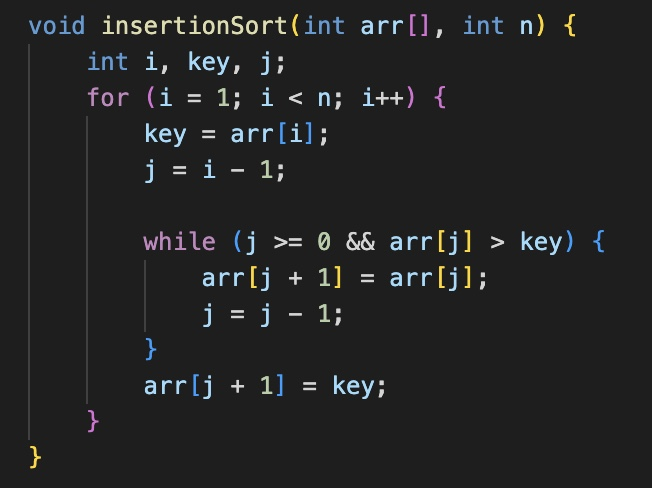
\includegraphics[width = 10cm]{Imagens/Insertion Sort/Imageminsert.jpg}
    \caption{Algoritmo Insertion Sort, criado pelo autor. }
    \label{fig:imagem_insert}
\end{figure}

\newpage
 Exemplo:\\
 Considere a seguinte entrada: 5, 2, 4, 6, 1, 3\\
 Saída esperada: 1, 2, 3, 4, 5, 6
\begin{figure}[htbp]
    \centering
    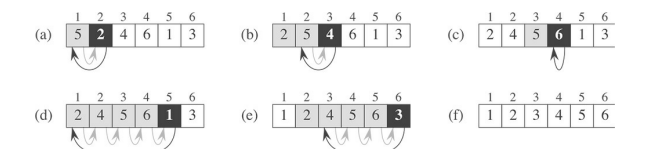
\includegraphics[width = 16cm]{Imagens/Insertion Sort/imagem1.png}
    \caption{Exemplo Insertion Sort retirado do livro Algoritmos: teoria e prática. }
    \label{grafico_insert}
\end{figure}

\cite{cormen2002}

O arranjo inicial a: [5, 2, 4, 6, 1, 3].
Primeira Iteração (índice 2, valor = 2):
comparamos 2 com 5 (à sua esquerda).
2 é menor, então trocamos.
Arranjo b: [2, 5, 4, 6, 1, 3]
Segunda Iteração (índice 3, valor = 4):
Comparamos 4 com 5.
4 é menor, então trocamos.
Arranjo c: [2, 4, 5, 6, 1, 3]
Terceira Iteração (índice 4, valor = 6):
Comparamos 6 com 5.
6 é maior, então não fazemos nada.
Arranjo d: [2, 4, 5, 6, 1, 3]
Quarta Iteração (índice 5, valor = 1):
Comparamos 1 com 6, 5, 4 e 2.
1 é menor que todos esses, então move-se para a primeira posição.
Arranjo e: [1, 2, 4, 5, 6, 3]
Quinta Iteração (índice 6, valor = 3):
Comparamos 3 com 6, 5, 4.
3 é menor que 6, 5 e 4, mas maior que 2.
Movemos 3 para a posição após 2.
Arranjo f: [1, 2, 3, 4, 5, 6]
Estado Final
Arranjo f: [1, 2, 3, 4, 5, 6].
        \subsection{Selection Sort}
		O Selection Sort é outro algoritmo de ordenação simples e intuitivo. Ele divide a lista de entrada em duas partes: a sublista de itens já ordenados e a sublista de itens ainda a serem ordenados. Em cada iteração, o algoritmo procura o menor (ou maior, dependendo da ordem desejada) elemento da sublista não ordenada e o troca com o primeiro elemento da sublista não ordenada. Este processo é repetido até que toda a lista esteja ordenada. Apesar de sua simplicidade, o Selection Sort pode ser ineficiente para listas muito grandes.

 \begin{figure}[h!]
    \centering
    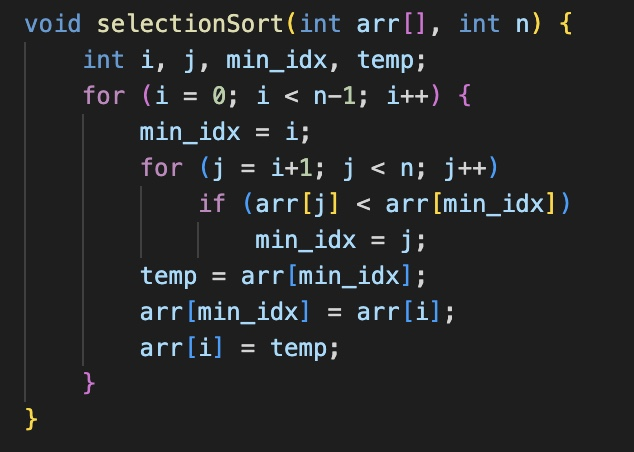
\includegraphics[width = 10cm]{Imagens/Selection Sort/Imagemselection.jpg}
    \caption{ALgoritmo Selection Sort, imagem criada pelo autor. }
    \label{imagem_insert}
\end{figure}

Exemplo: 

Vamos considerar o seguinte array como exemplo \cite{site2023}: arr[]= {64, 25, 12, 22, 11}
\par Primeiro passo conforme à figura \ref{fig:enter-label}: para a primeira posição na matriz, toda a matriz é percorrida do índice 0 ao 4, subsequencialmente. A primeira posição onde 64 está armazenado atualmente, depois de percorrer todo o array, chega a conclusão de que o 11 é o menor valor. Assim, substitua o 64 por 1. Após uma iteração, 11, que é o menor valor da matriz, passa a aparecer na primeira posição da lista ordenada. 

\begin{figure} [h!]
    \centering
    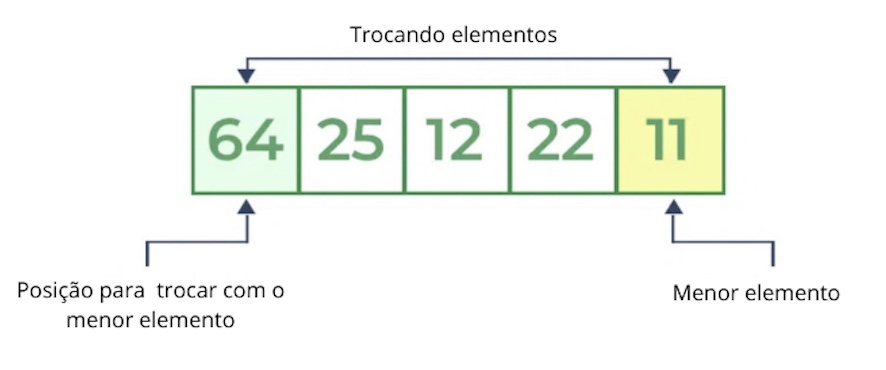
\includegraphics[width = 10cm]{Imagens/Selection Sort/Imagem 27-09-2023 às 16.06.jpeg}
    \caption{Selection Sort | Trocando o 1º elemento pelo mínimo do array}
    \label{fig:enter-label}
\end{figure}

\par Segundo passo conforme à figura \ref{fig:exemplo2}: para a segunda opção, onde o 25 está ocupando, percorra novamente todo o array. Após percorrer, descobrimos que 12 é o segundo menor valor do array e deve aparecer na segunda opção, portanto realiza a troca desses valores.

\begin{figure}[h!]
    \centering
    \includegraphics[width = 10cm]{Imagens/Selection Sort/Captura de Tela 2023-09-27 às 16.15.34.png}
    \caption{Selection Sort | trocando i=1 pelo próximo elemento mínimo}
    \label{fig:exemplo2}
\end{figure}
\newpage
\par Terceiro passo conforme à figura \ref{fig:exemplo3}: agora, para o terceiro lugar, onde 25 está presente, percorra novamente o restante do array e encontre o terceiro menor valor presente no array. Durante o processo, 22 acabou sendo o terceiro menor valor e deveria aparecer na terceira posição do array, portantanto troque 22 pelo elemento presente na terceira posição.

\begin{figure}[h!]
    \centering
    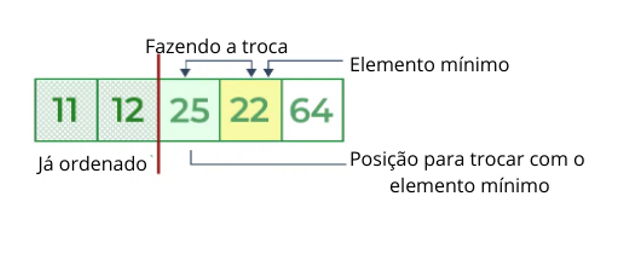
\includegraphics[width = 10cm]{Imagens/Selection Sort/image1.png}
    \caption{Selection Sort | trocando i=2 pelo próximo elemento mínimo}
    \label{fig:exemplo3}
\end{figure}

\par Quarto passo conforme à figura \ref{fig:exemplo4}: da mesma forma que os anteriores, percorra o resto da matriz e encontre o quarto menor elemento da matriz. Como 25 é o quarto valor mais baixo, ele ficará na mesma posição.

\begin{figure}[h!]
    \centering
    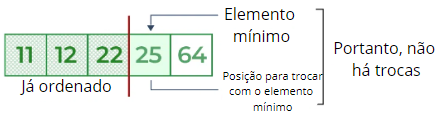
\includegraphics[width = 10cm]{Imagens/Selection Sort/image2.png}
    \caption{Selection Sort | trocando i=3 pelo próximo elemento mínim}
    \label{fig:exemplo4}
\end{figure}

\par Quinto passo conforma à figura \ref{fig:exemplo5}: por fim, o maior valor presente no arrray é automaticamente colocado na última posição do array, a matriz resultante é a matriz ordenada.

\begin{figure}[h!]
    \centering
    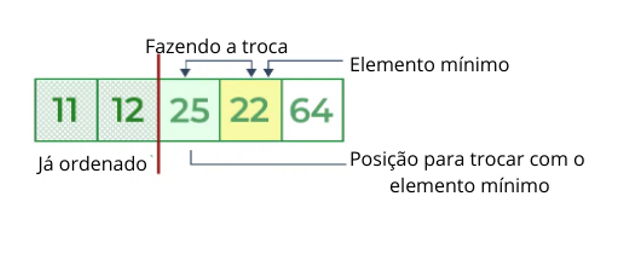
\includegraphics[width = 10cm]{Imagens/Selection Sort/image1.png}
    \caption{Selection Sort | Matriz ordenada}
    \label{fig:exemplo5}
\end{figure}
        \subsection{Shell Sort}
		O Shell Sort é um algoritmo de ordenação mais complexo e uma extensão do Insertion Sort. Ele começa ordenando elementos que estão distantes entre si e progressivamente reduz a distância entre os elementos a serem comparados\cite{sedgewick1986shell}. Em cada etapa, ele usa o Insertion Sort para ordenar os pares de elementos escolhidos, até que, na última etapa, a lista inteira é ordenada usando o Insertion Sort. O Shell Sort é mais eficiente em comparação com os algoritmos de ordenação simples, especialmente para listas grandes e não ordenadas, devido à sua abordagem de redução de distância.

\begin{figure}[h!]
    \centering
    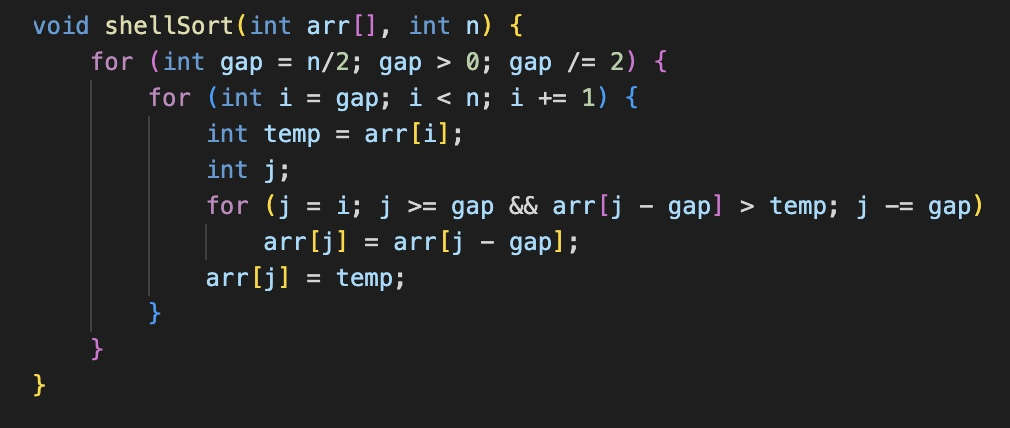
\includegraphics[width = 10cm]{Imagens/Shell Sort/ImagemShell.jpg}
    \caption{ALgoritmo Shell Sort, imagem criada pelo autor.}
    \label{fig:imagemshell}
\end{figure}

Exemplo prático Shell Sort \cite{siteShell}:
Suponha que precisamos classificar o seguinte array da figura \ref{fig:ex1}:
\begin{figure}[h!]
    \centering
    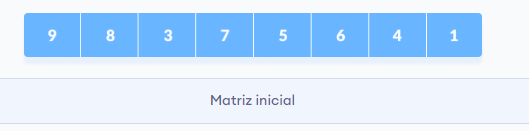
\includegraphics[width = 10cm]{Imagens/Shell Sort/ex1.png}
    \caption{Matriz Inicial}
    \label{fig:ex1}
\end{figure}

\par \newpage No primeiro loop, se o tamanho do array for N = 8 então, os elementos que estão no intervalo de N/2 = 4 são comparados e trocados se não estiverem em ordem.
O 0º elemento é comparado com o4ºelemento.
Se o 0º elemento for maior que o4ºum então, o4ºo elemento é armazenado primeiro na temp variável e o 0º elemento (ou seja, o elemento maior) é armazenado na 4º posição e o elemento armazenado tempé armazenado na 0º posição.

\begin{figure}[h!]
    \centering
    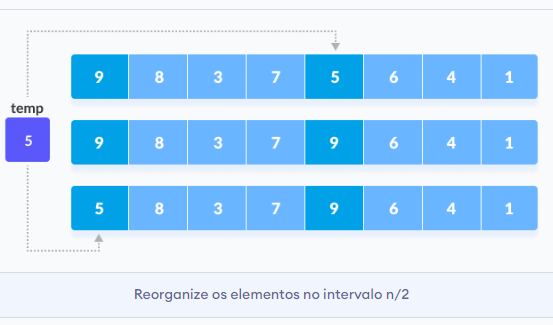
\includegraphics[width = 10cm]{Imagens/Shell Sort/ex2.png}
    \caption{Reorganize os elementos no intervalo n/2}
    \label{fig:ex2}
\end{figure}

\par Este processo continua para todos os elementos restantes.

\begin{figure}[h!]
    \centering
    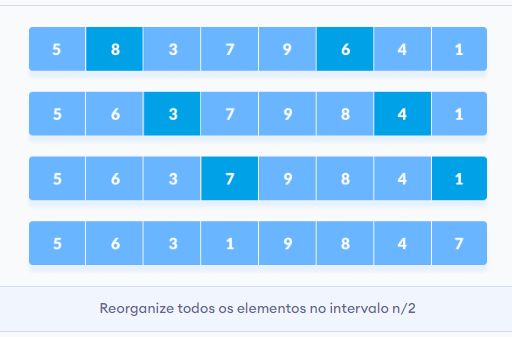
\includegraphics[width = 10cm]{Imagens/Shell Sort/ex3.png}
    \caption{Reorganize os elementos no intervalo n/2}
    \label{fig:ex3}
\end{figure}

\par No segundo loop, um intervalo de N/4 = 8/4 = 2é obtido e novamente os elementos situados nesses intervalos são classificados.

\begin{figure}[h!]
    \centering
    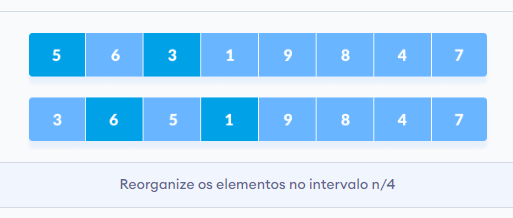
\includegraphics[width = 10cm]{Imagens/Shell Sort/ex4.png}
    \caption{Reorganize os elementos no intervalo n/4}
    \label{fig:ex4}
\end{figure}

\begin{figure}[h!]
    \centering
    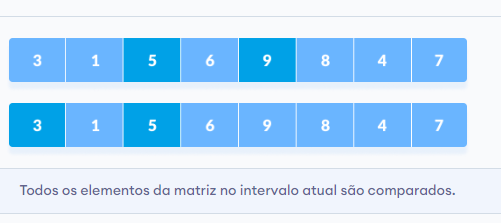
\includegraphics[width = 10cm]{Imagens/Shell Sort/ex5.png}
    \caption{Todos os elementos da matriz no intervalo atual são comparados.}
    \label{fig:ex5}
\end{figure}

\par\newpage Os elementos em 4º e 2º posição são comparadas. Os elementos em2ºe 0tha posição também são comparadas. Todos os elementos da matriz no intervalo atual são comparados. O mesmo processo continua para os elementos restantes.

\begin{figure}[h!]
    \centering
    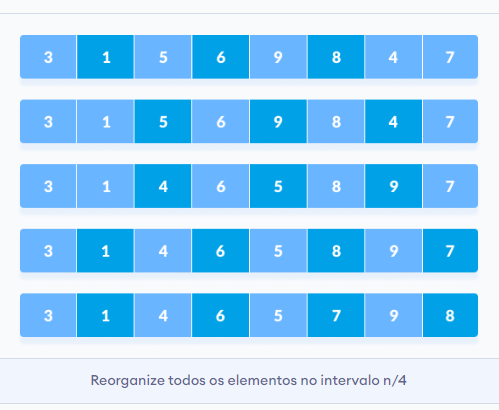
\includegraphics[width = 10cm]{Imagens/Shell Sort/ex6.png}
    \caption{Reorganize todos os elementos no intervalo n/4.}
    \label{fig:ex6}
\end{figure}

 \par E finalmente, quando o intervalo é N/8 = 8/8 =1 então, os elementos da matriz situados no intervalo de 1 são classificados. A matriz agora está completamente classificada \ref{fig:ex7}.

\begin{figure}[h!]
    \centering
    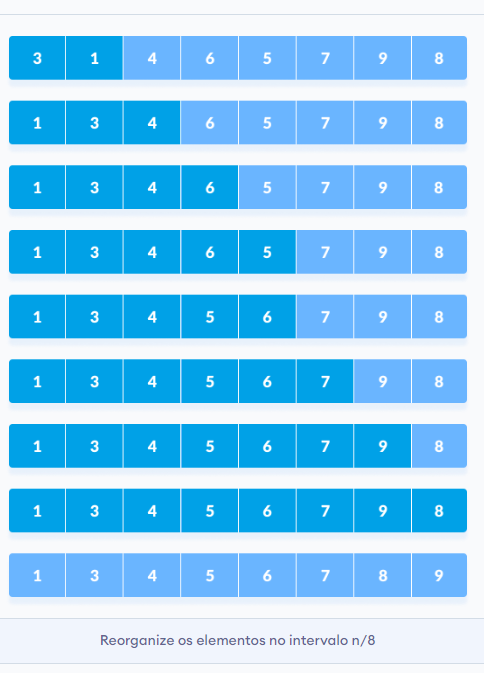
\includegraphics[width = 7cm]{Imagens/Shell Sort/ex7.png}
    \caption{Reorganize os elementos no intervalo n/8.}
    \label{fig:ex7}
\end{figure}
 


        \newpage
        \subsection{Bubble Sort}
		O Bubble Sort é um algoritmo de ordenação simples onde a lista é percorrida da primeira até a última posição, comparando pares de elementos adjacentes e trocando-os se estiverem na ordem errada\cite{cormen2009introduction}. Este processo é repetido até que a lista esteja ordenada. Devido à sua natureza de comparação e troca, o Bubble Sort não é o método mais eficiente para listas grandes, mas sua implementação é direta e intuitiva. O algoritmo não
tem uma condição de parada, por isso as comparações são realizadas uma por uma mesmo array estando ordenado assim aumentando o seu tempo de execução.

\begin{figure}[h!]
    \centering
    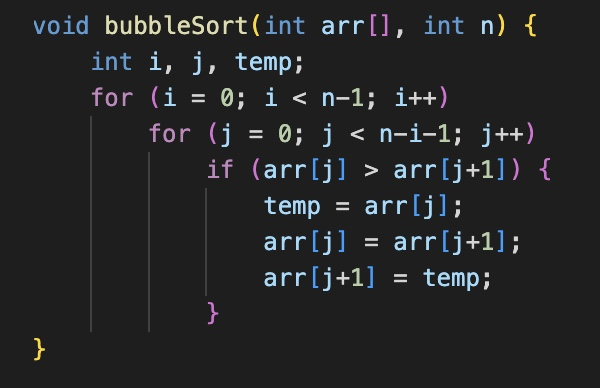
\includegraphics[width = 10cm]{Imagens/Bubble Sort/ImagemBubble.jpg}
    \caption{ALgoritmo Bubble Sort, imagem criada pelo autor.}
    \label{fig:imagembubble}
\end{figure}

Vamos entender o funcionamento do Bubble Sort com o seguinte exemplo \cite{sitebubble}: 
Entrada: arr[] = {6, 3, 0, 5}
Primeiro passo: O maior elemento é colocado em sua posição correta, ou seja, no final do array conforme na Figura \ref{fig:b1}.

\begin{figure}[h!]
    \centering
    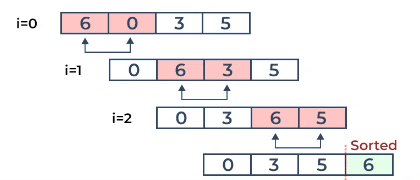
\includegraphics[width = 10cm]{Imagens/Bubble Sort/bubble1.png}
    \caption{Bubble Sort: colocando o maior elemento na posição correta.}
    \label{fig:b1}
\end{figure}

Segundo passo: Coloque o segundo maior elemento na posição correta, conforme na figura \ref{fig:b2}.

\begin{figure}[h!]
    \centering
    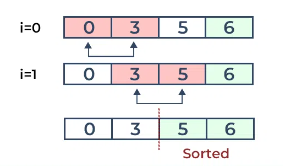
\includegraphics[width = 10cm]{Imagens/Bubble Sort/bubble2.png}
    \caption{Bubble Sort: colocando o segundo maior elemento na posição correta.}
    \label{fig:b2}
\end{figure}

Terceiro passo: Coloque os dois elementos restantes em suas devidas posições como mostra a figura \ref{fig:b3}.

\begin{figure}[h!]
    \centering
    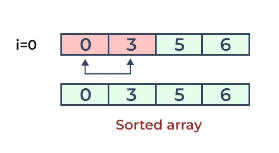
\includegraphics[width = 10cm]{Imagens/Bubble Sort/bubble3.png}
    \caption{Bubble Sort: colocando os elementos restantes em suas posições corretas.}
    \label{fig:b3}
\end{figure}
		\newpage
        \subsection{Merge Sort}
		O Merge Sort é um algoritmo de ordenação bastante diferente do Insertion Sort, tanto em abordagem quanto em eficiência. Enquanto o Insertion Sort constrói a lista ordenada um item por vez, inserindo cada novo elemento em sua posição correta dentro da parte já ordenada, o Merge Sort adota uma estratégia de "dividir para conquistar"\cite{cyberini2018mergesort}.

 \begin{figure}[H]
    \centering
    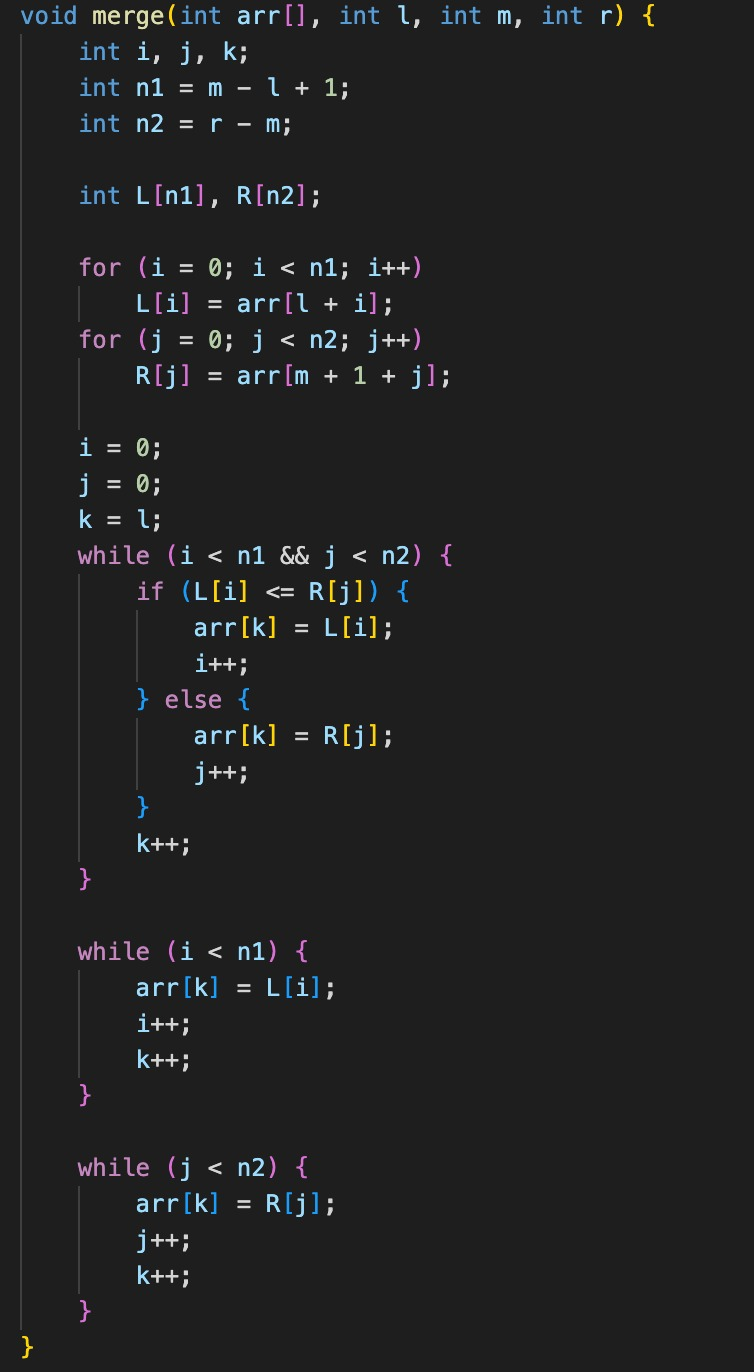
\includegraphics[width = 6cm]{Imagens/Merge Sort/WhatsApp Image 2023-11-13 at 21.41.34.jpeg}
    \caption{ALgoritmo Merge Sort, imagem criada pelo autor. }
    \label{imagem_merge}
\end{figure}

 \begin{figure}[H]
    \centering
    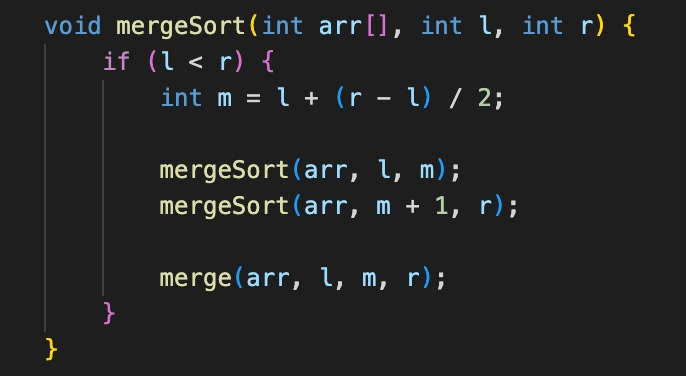
\includegraphics[width = 6cm]{Imagens/Merge Sort/WhatsApp Image 2023-11-13 at 21.41.34 (1).jpeg}
    \caption{ALgoritmo Merge Sort, imagem criada pelo autor. }
    \label{imagem_merge}
\end{figure}

\par A seguir, um exemplo do funcionamento do Merge Sort:

 \begin{figure}[H]
    \centering
    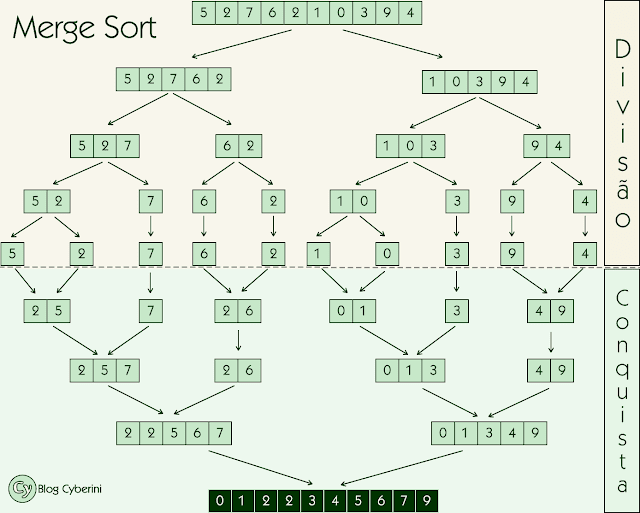
\includegraphics[width = 6cm]{Imagens/Merge Sort/diagrama-merge-sort.png}
    \caption{Exemplo do Merge Sort\cite{cyberini2018mergesort}. }
    \label{imagem_digrama}
\end{figure}

Como mostrado na Figura~\ref{fig:imagem_diagrama}, o Merge Sort funciona da seguinte maneira: 
1-Divisão Recursiva: O Merge Sort começa dividindo o conjunto de dados em duas metades iguais (ou quase iguais). Essa divisão continua recursivamente até que cada subconjunto contenha apenas um elemento (ou nenhum, se o conjunto inicial for vazio).

2-Fusão e Ordenação: Após a divisão, o algoritmo começa a combinar os subconjuntos, ordenando-os no processo. Dois subconjuntos são comparados elemento a elemento, e os elementos são ordenados e mesclados em um novo subconjunto. Esse processo de fusão continua até que todos os subconjuntos pequenos sejam combinados de volta em um único conjunto ordenado.

        \subsection{Quick Sort}
		O Quick Sort é uma técnica de ordenação que utiliza a estratégia de divisão e conquista. Essa abordagem consiste em reorganizar a lista de tal maneira que os elementos menores que um elemento selecionado, chamado pivô, fiquem à sua esquerda, enquanto os maiores ficam à direita. Este processo é realizado de maneira recursiva, diminuindo progressivamente o tamanho das listas a serem ordenadas\cite{devto_quick_sort}.

Os passos fundamentais são:

1- Seleção do Pivô: Um elemento da lista é escolhido para ser o pivô.
2- Particionamento: A lista é reorganizada de forma que todos os elementos à esquerda do pivô sejam menores que ele, e todos à direita sejam maiores. Após essa etapa, o pivô estará em sua posição definitiva, resultando em duas sublistas não ordenadas. Esta etapa é crucial para o processo.
3- Ordenação Recursiva: As sublistas contendo os elementos menores e maiores que o pivô são ordenadas recursivamente.
4- Caso Base: A recursão tem como caso base listas de tamanho zero ou um, que naturalmente estão ordenadas. O algoritmo termina quando todas as sublistas alcançam esse estado.

A eficiência do Quick Sort é significativamente influenciada pela escolha do pivô e pela implementação do processo de particionamento. Diferentes métodos para estas etapas podem resultar em variações substanciais no desempenho do algoritmo, especialmente em diferentes tipos de conjuntos de dados. Neste trabalho iremos fazer testes com 4 tipos diferentes de pivô: 
Versão 1: Pivô como primeiro elemento.
\begin{figure}[H]
    \centering
    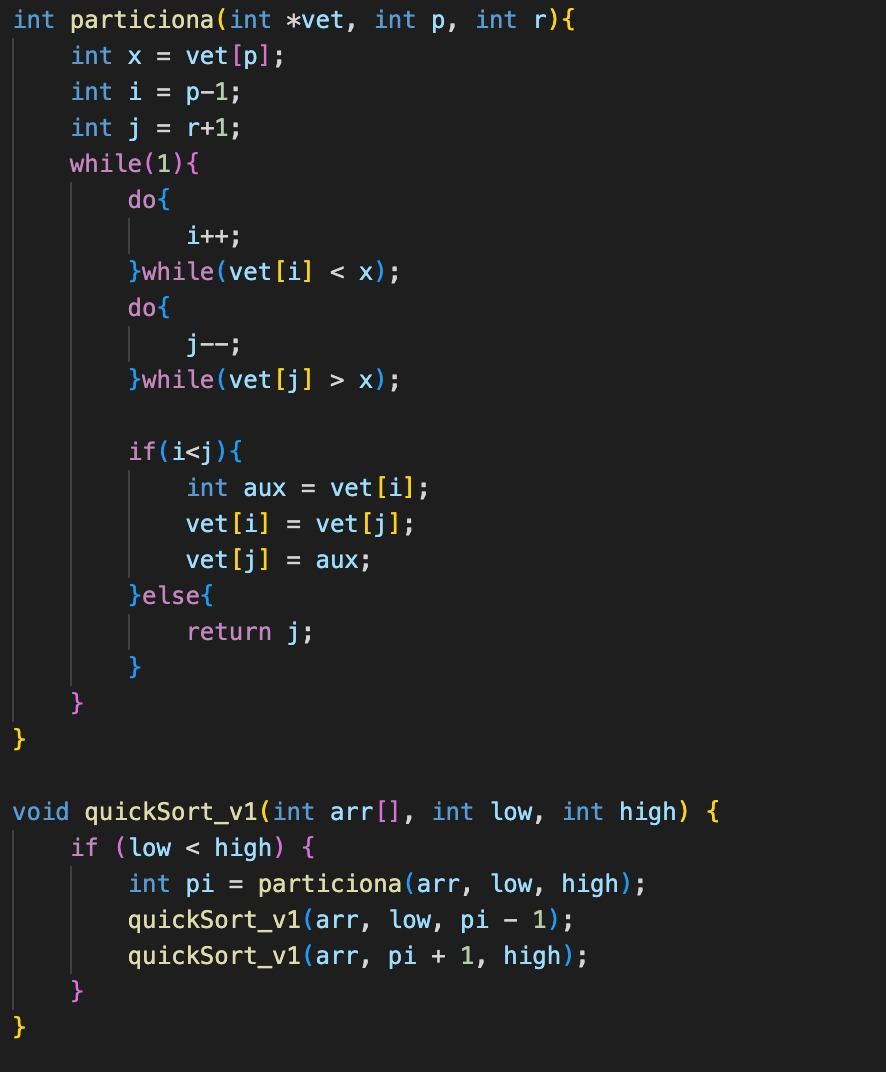
\includegraphics[width = 10cm]{Imagens/Quick Sort/quick1.jpeg}
    \caption{Quick Sort 1}
    \label{grafico_insert}
\end{figure}
Esta é a versão clássica do Quick Sort, onde o primeiro elemento do segmento do array que está sendo ordenado é escolhido como pivô. O objetivo do pivô é ajudar na divisão do array em duas partes, onde um lado contém elementos menores que o pivô e o outro lado contém elementos maiores. Esta versão é simples e eficaz, mas pode ter desempenho subótimo em arrays já ordenados ou quase ordenados.
Versão 2: Pivô como média dos elementos.
\begin{figure}[H]
    \centering
    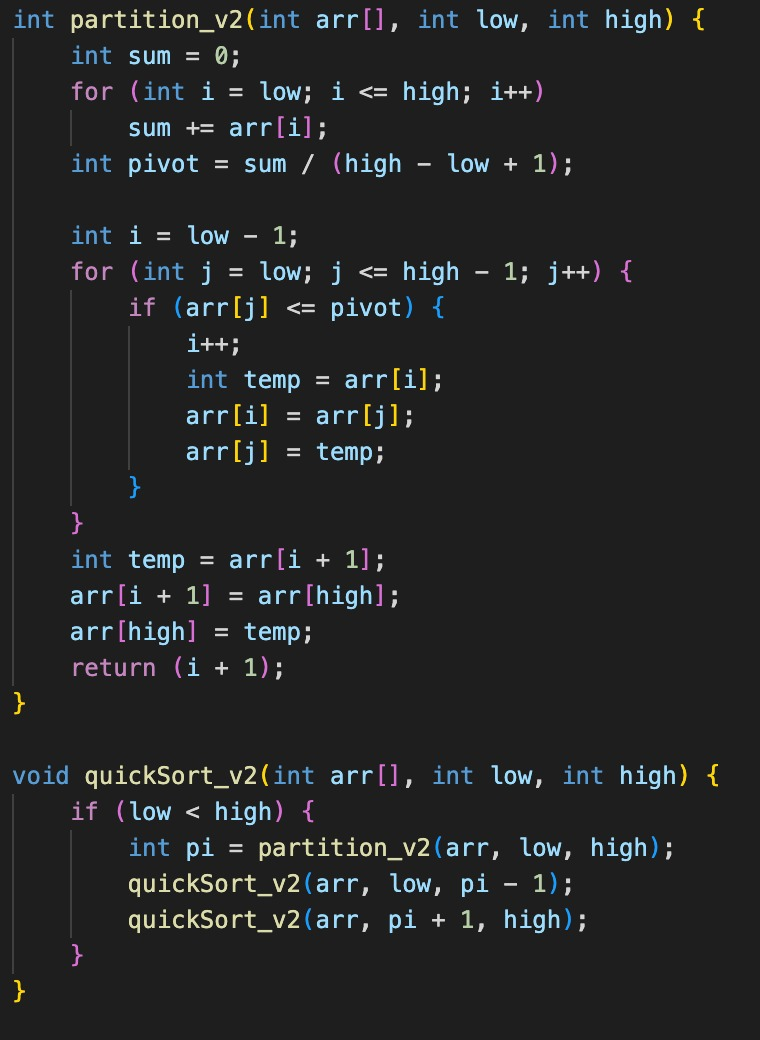
\includegraphics[width = 10cm]{Imagens/Quick Sort/quick2.jpeg}
    \caption{Quick Sort 2}
    \label{grafico_insert}
\end{figure}
Nesta versão, o pivô é escolhido como a média dos valores do segmento do array a ser ordenado. Ao usar a média, busca-se um valor de pivô mais representativo do conjunto de dados, o que pode resultar em uma divisão mais equilibrada do array, especialmente em casos onde os dados têm uma distribuição mais uniforme. Esta abordagem pode melhorar o desempenho em comparação com a escolha do primeiro elemento como pivô.
Versão 3: Pivô como mediana de três elementos.
\begin{figure}[H]
    \centering
    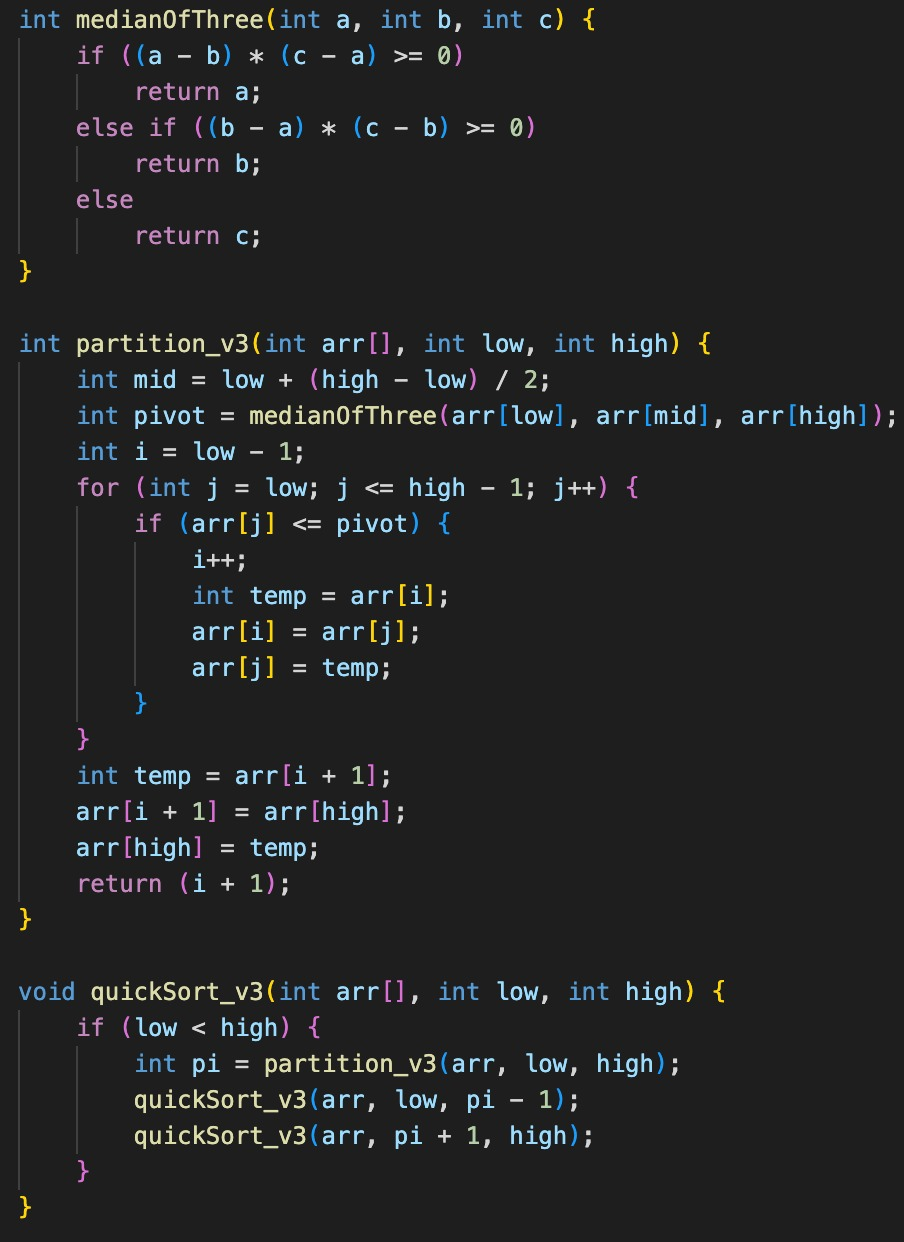
\includegraphics[width = 10cm]{Imagens/Quick Sort/quick3.jpeg}
    \caption{Quick Sort 3}
    \label{grafico_insert}
\end{figure}
Aqui, o pivô é escolhido como a mediana de três elementos selecionados: o primeiro, o último e o elemento do meio do segmento do array. Esta estratégia é uma tentativa de encontrar um bom pivô que seja mais representativo do array inteiro, reduzindo a chance de pior caso (como em arrays já ordenados). Escolher a mediana desses três elementos é um bom equilíbrio entre o custo de cálculo do pivô e a eficiência na divisão do array.
Versão 4: Pivô escolhido aleatoriamente.
\begin{figure}[H]
    \centering
    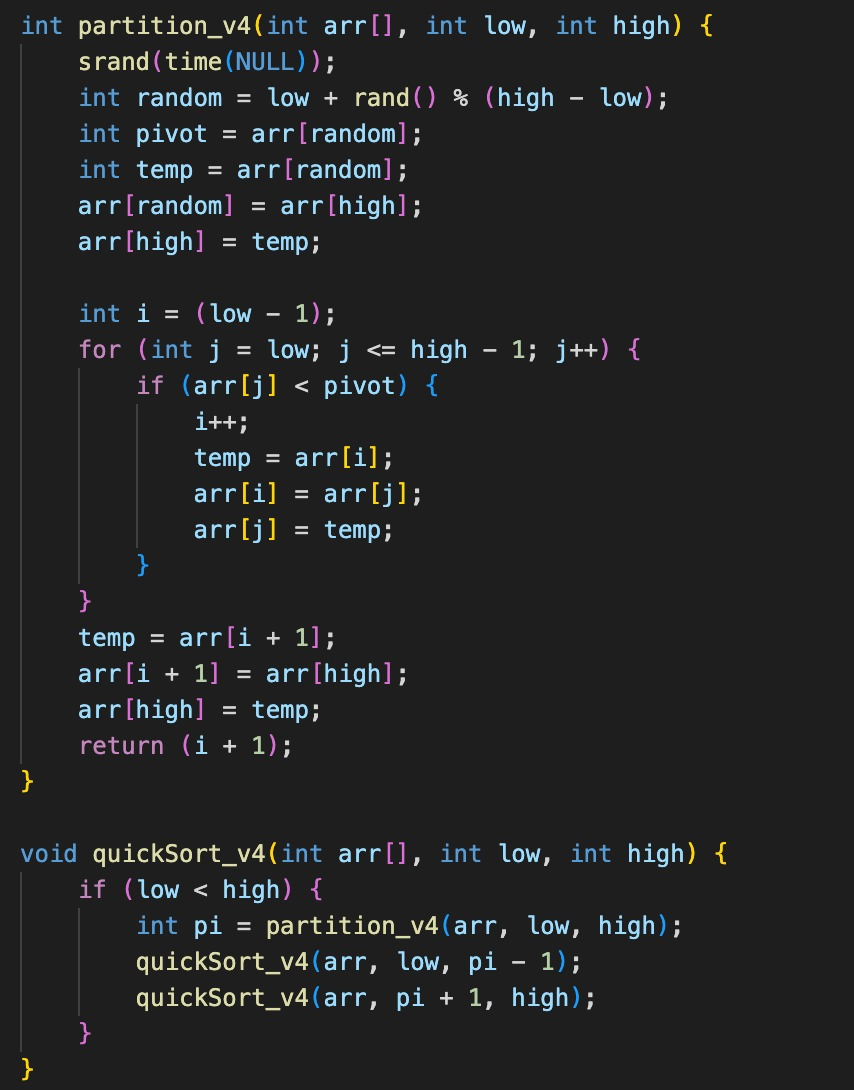
\includegraphics[width = 10cm]{Imagens/Quick Sort/quick4.jpeg}
    \caption{Quick Sort 4}
    \label{grafico_insert}
\end{figure}
Nesta abordagem, o pivô é escolhido de forma aleatória. Esta estratégia ajuda a garantir que, em média, o array seja dividido de forma relativamente equilibrada, reduzindo a probabilidade de pior caso independente da ordenação inicial do array. A escolha aleatória é particularmente útil para evitar o pior caso em arrays que possam ter alguma ordem específica ou padrão.
        \subsection{HeapSort}
		O HeapSort é um eficiente algoritmo de ordenação que se baseia no conceito de árvores binárias, especificamente na estrutura de dados conhecida como Heap. Desenvolvido em 1964 por Robert W. Floyd e J.W.J. Williams, este método compartilha a Ordem de Complexidade O(n log n) com outros algoritmos eficientes, mas se distingue pelo uso de heaps para otimizar o processo de seleção dos itens.\cite{mello2002ordenacao}

Funcionamento do HeapSort:
O processo do HeapSort inicia com a construção de um heap, que pode ser um heap máximo (max heap) ou mínimo (min heap). Em um max heap, cada nó pai tem um valor maior que o de seus filhos, enquanto em um min heap, cada nó pai tem um valor menor. Isso coloca o maior (ou menor) valor na raiz da árvore, que corresponde ao primeiro elemento do array.\cite{lopes2005heap}

O algoritmo então repete o processo de remoção do nó raiz (o maior ou menor elemento, dependendo do tipo de heap), reposicionando o último elemento do heap na raiz e reajustando a estrutura para manter as propriedades do heap. Esse processo de reajuste, ou "heapify", é essencial para manter a ordem correta durante a ordenação.

 \begin{figure}[H]
    \centering
    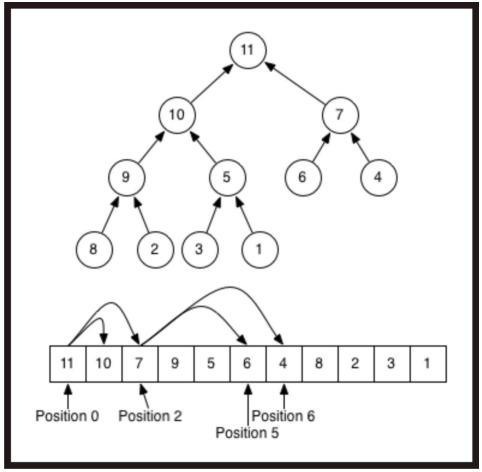
\includegraphics[width = 6cm]{Imagens/Heap Sort/image.png}
    \caption{Ilustração de um Heap máximo\cite{lopes2005heap}. }
    \label{imagem_heap}
\end{figure}

Os algoritmos para implementar as operações sobre o heap operam ao longo de um dos caminhos da árvore, a partir da raiz até o nível mais profundo da árvore. Para o HeapSort, são necessárias apenas duas operações com o heap: \textit{Remake}, que refaz a estrutura, e \textit{Build}, que a constrói. Eles são apresentados no Programa 1.

\begin{verbatim}
Programa 1: Operações com Heap necessárias ao HeapSort.
void SortMethods::ReMake(long Left, long Right, TItem *Array) {
    long i = Left;
    long j;
    TItem aux;
    j = i * 2;
    aux = Array[i];
    while (j <= Right) {
        if (j < Right) {
            this->mComparations++;
            if (Array[j].Key < Array[j + 1].Key)
                j++;
        }
        this->mComparations++;
        if (aux.Key >= Array[j].Key)
            break;
        Array[i] = Array[j];
        i = j;
        j = i * 2;
        this->mMoviments++;
    }
    Array[i] = aux;
    this->mMoviments++;
}

void SortMethods::Build(TItem *Array, long n) {
    long Left;
    Left = n / 2 + 1;
    while (Left > 1) {
        Left--;
        ReMake(Left, n, Array);
    }
}
\end{verbatim}

O método de Ordenação HeapSort é iniciado com um heap obtido através do método \textit{Build}.

\begin{verbatim}
Programa 2: Método HeapSort.
void SortMethods::HeapSort(TItem *Array, long n) {
    long Left, Right;
    TItem aux;
    CTimer *Timer = new CTimer();
    this->ClearAll();
    Timer->start();
    this->Build(Array, n);
    Left = 0;
    Right = n-1;
    while (Right > 0) {
        aux = Array[0];
        Array[0] = Array[Right];
        Array[Right] = aux;
        this->mMoviments++;
        Right--;
        this->ReMake(Left, Right, Array);
    }
    Timer->stop();
    this->mTime = Timer->getElapsedTime();
}
\end{verbatim}

Depois pega-se o item na posição 0 do vetor(raiz do heap) e troca-se com o
item que está na posição n do vetor, como apresentado no Programa 2. A seguir,
basta usar o método ReMake com o restante dos itens. A Figura 29\ref{fig:imagem_heap1} ilustra o
funcionamento deste método.

 \begin{figure}[H]
    \centering
    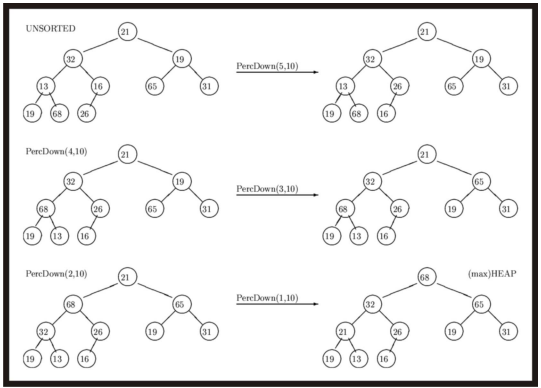
\includegraphics[width = 6cm]{Imagens/Heap Sort/heapheao.png}
    \caption{Ilustração do funcionamento do algoritmo HeapSort. }
    \label{imagem_heap1}
\end{figure}


        \subsection{Fila de Prioridades}
		Filas de prioridades são estruturas de dados essenciais que permitem o armazenamento de elementos com a capacidade de recuperar rapidamente o item com a maior (ou menor) prioridade. Em um \textit{min-heap}, a prioridade é determinada pela chave do elemento, onde uma chave menor indica uma prioridade mais alta.

\subsection*{Operações Fundamentais}

\begin{itemize}
  \item \textbf{heap\_minimum}: Esta operação retorna o elemento com a menor chave no min-heap, que é sempre o elemento na raiz da árvore. Sua complexidade é $O(1)$, pois o elemento mínimo é acessado diretamente.
  
  \item \textbf{heap\_extract\_min}: Remove e retorna o elemento com a menor chave no min-heap. A complexidade desta operação é $O(\log n)$ devido ao processo de reestruturação do heap após a remoção do elemento mínimo.
  
  \item \textbf{heap\_increase\_key}: Aumenta o valor da chave de um elemento em um min-heap. Após o aumento, o heap é ajustado para manter a propriedade de min-heap, o que leva a uma complexidade de $O(\log n)$.
  
  \item \textbf{min\_heap\_insert}: Insere um novo elemento no min-heap. A inserção pode exigir a reestruturação do heap para manter a propriedade de ordenação, resultando em uma complexidade de $O(\log n)$.
\end{itemize}

Essas operações permitem que as filas de prioridades baseadas em min-heap ofereçam uma maneira eficiente de acessar e modificar elementos com base em suas prioridades, mantendo uma complexidade logarítmica para as operações mais custosas.

\begin{figure}[H]
    \centering
    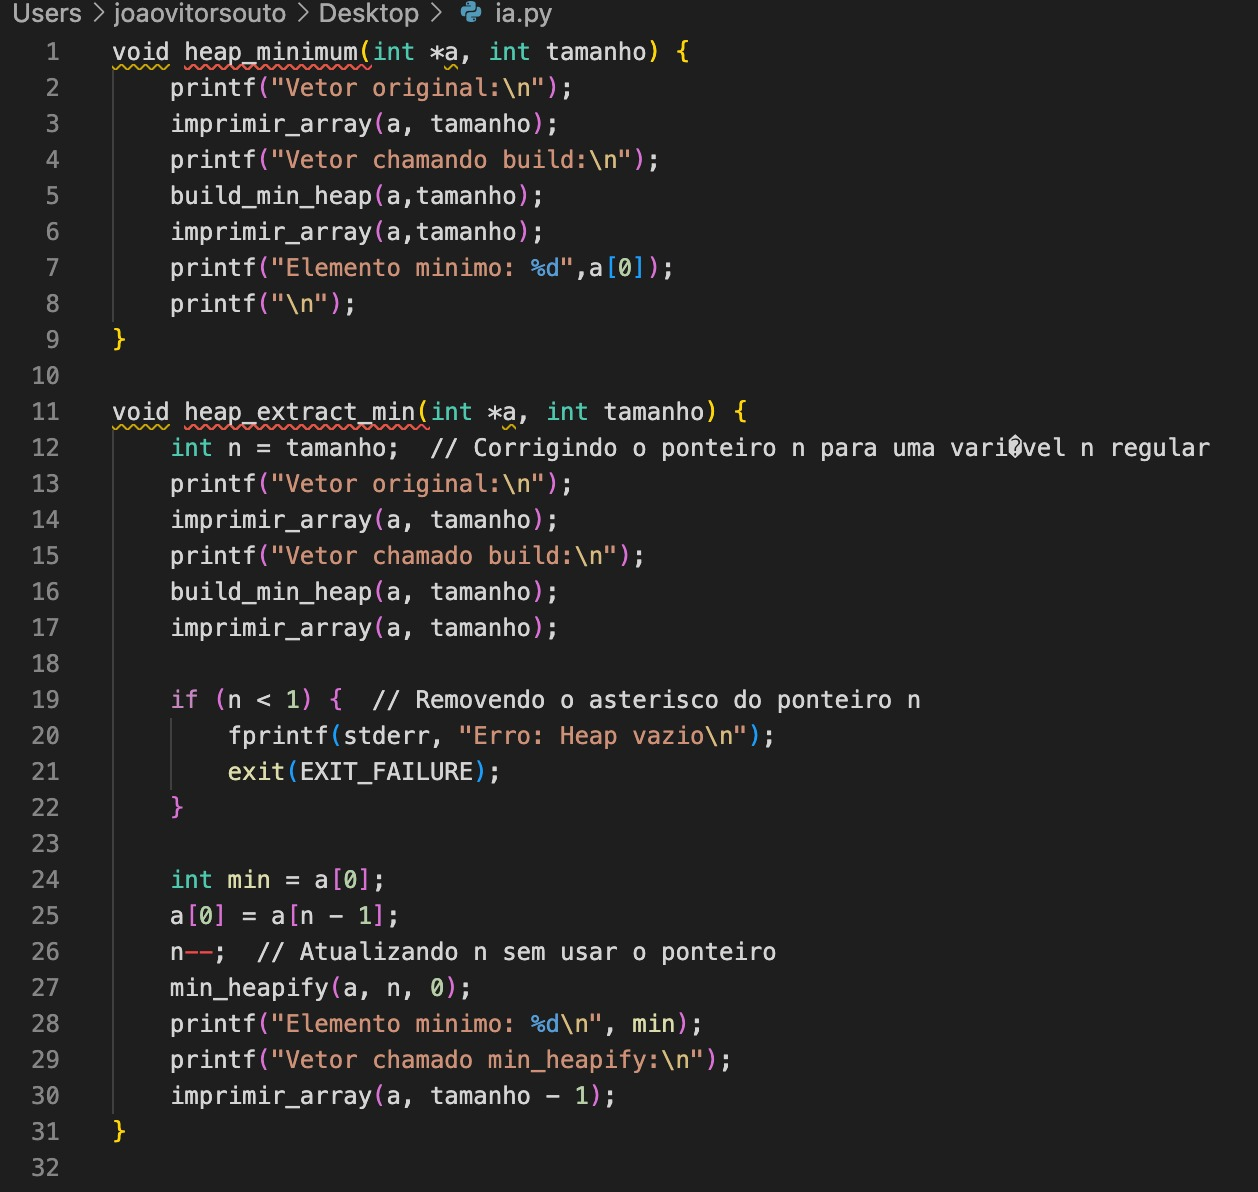
\includegraphics[width = 10cm]{Imagens/fila/98cf0803-8396-443a-a626-22850b4a8a54.jpg}
    \caption{Código Fila de Prioridade}
    \label{grafico_insert}
\end{figure}

\begin{figure}[H]
    \centering
    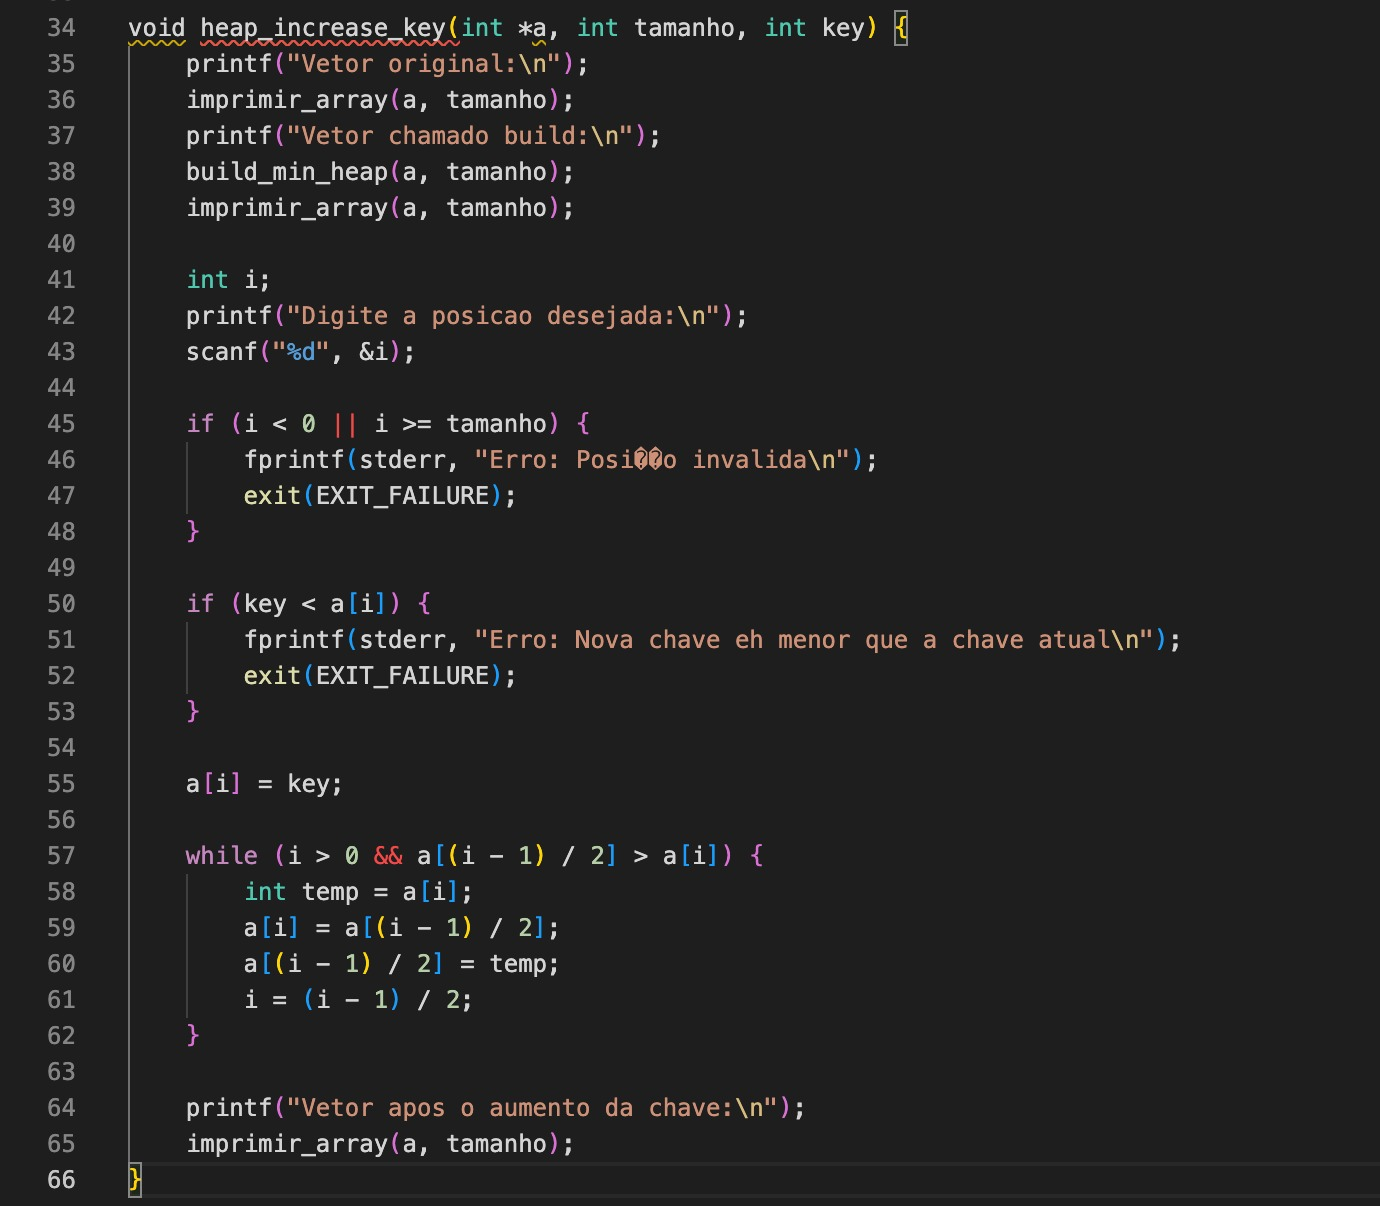
\includegraphics[width = 10cm]{Imagens/fila/5f8a8050-b74b-4d6d-8770-07522b37a09a.jpg}
    \caption{Código Fila de Prioridade 2}
    \label{grafico_insert}
\end{figure}
         
            \section{ANÁLISE DE COMPLEXIDADE}
		\subsection{Insertion Sort}
		
Análise de Insertion Sort: A análise começa com uma descrição detalhada dos custos associados a cada linha do pseudo-código de Insertion Sort. Ela também considera o número de vezes que cada linha é executada, especialmente focando no teste do laço while\cite{cormen2002}.

A análise pode eventualmente ser simplificada, passando de uma fórmula complexa com múltiplos termos para uma notação mais gerenciável e intuitiva, como a notação O big (O), que é mais fácil de usar para comparar a eficiência de diferentes algoritmos.

\begin{figure}[htbp]
    \centering
    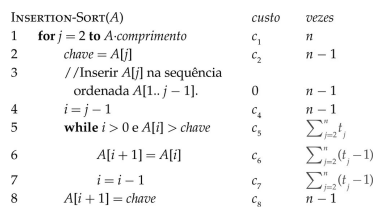
\includegraphics[width = 10cm]{Imagens/Insertion Sort/custosINSERT.png}
    \caption{Tabela sobre o custo do Insertion Sort}
    \label{grafico_insert}
\end{figure}

\begin{figure}[h!]
    \centering
    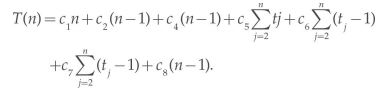
\includegraphics[width = 10cm]{Imagens/Insertion Sort/formula.png}
    \caption{Fórmula para calcular T(n) Insertion Sort.}
    \label{grafico_insert}
\end{figure}



MELHOR CASO: O melhor caso ocorre quando o arranjo já está ordenado. Neste cenário, o algoritmo percorre o arranjo uma única vez, tornando sua complexidade de tempo O(n) conforme equação \eqref{eq:funcao_linear}. 

\begin{equation}
T(n) = C_1n + C_2(n-1) + C_3(n-1) + C_4(n-1) + C_7(n-1)
\end{equation}

Aplicando a distributiva, temos:

\begin{align}
T(n) &= C_1n + (C_2n - C_2) + (C_3n - C_3) + (C_4n - C_4) + (C_7n - C_7) \\
     &= (C_1 + C_2 + C_3 + C_4 + C_7)n - (C_2 + C_3 + C_4 + C_7)
\end{align}

Assim, o resultado é uma função linear:

\begin{equation}
T(n) = An - B \quad \text{(Função linear)}
\label{eq:funcao_linear}
\end{equation}

PIOR CASO: O pior caso acontece quando o arranjo está ordenado em ordem decrescente. Isso força o algoritmo a fazer o máximo de comparações e movimentações, resultando em uma complexidade de tempo O($ n^2 $) conforme equação \eqref{eq:funcao_quadratica}.

\begin{equation}
T(n) = C_1n + C_2(n-1) + C_3(n-1) + C_4\left(\sum_{j=2}^{n} T_j \right) + C_5\left(\sum_{j=2}^{n} (T_j - 1) \right) + C_6\left(\sum_{j=2}^{n} (T_j - 1) \right) + C_7(n - 1)
\end{equation}

que resulta em

\begin{equation}
T(n) = An^2 + Bn + C \quad \text{(Função quadrática)}
\label{eq:funcao_quadratica}
\end{equation}


CASO MÉDIO: Este é o cenário mais representativo para a maioria das aplicações práticas. No caso médio, a complexidade de tempo também é O($ n^2 $), mas o número de comparações e movimentações é, em média, menor do que no pior caso.
Cálculo médio caso: \begin{equation}
T(n) = C_1n + C_2(n-1) + C_3(n-1) + C_4\left(\sum_{j=2}^{n} T_j\right) + C_5\left(\sum_{j=2}^{n}(T_j - 1)\right) + C_6\left(\sum_{j=2}^{n}(T_j - 1)\right) + C_7(n - 1)
\end{equation}
Que resulta em T(n)=A$ n^2 $ + Bn + C(Função quadrática).


        \newpage
  	\subsection{Selection Sort}
		A complexidade do Selection Sort é a mesma, $O(n^2)$, para os três casos: melhor, pior e médio caso, pois seu algoritmo não contém condição de parada.

Fórmula Geral \ref{eq:formula_geral}:
\begin{equation}
T(n) = C_1n + C_2(n-1) + C_3\left(\sum_{j=2}^{n} T_j \right) + C_4\left(\sum_{j=2}^{n} (T_j - 1) \right) + C_5\left(\sum_{j=2}^{n} (T_j - 1) \right) + C_6(n-1)
\label{eq:formula_geral}
\end{equation}

\begin{table}[H] 
\centering
\begin{tabular}{|c|c|c|c|}
    \hline
    \textbf{Linhas} & \textbf{Algoritmo} & \textbf{Custo} & \textbf{Vezes} \\\hline
    1 & para \(i = 1\) até \textit{comprimento} - 1 & \(C_1\) & \(n\) \\
    2 & \quad menor = i & \(C_2\) & \(n-1\) \\
    3 & \quad para \(j = i + 1\) até \textit{comprimento} & \(C_3\) & \(\sum_{j=2}^{n} T_j\) \\
    4 & \quad se \(A[j] < A[\text{menor}]\) & \(C_4\) & \(\sum_{j=2}^{n} (T_j - 1)\) \\
    5 & \quad menor = j & \(C_5\) & \(\sum_{j=2}^{n} (T_j - 1)\) \\
    6 & \textit{swap}(A[j], A[menor]) & \(C_6\) & \(n-1\) \\
    \hline
\end{tabular}
\caption{Tabela de complexidade do Selection Sort.}
\label{tab:complexidade_selection}
\end{table}



\paragraph{PIOR CASO:}
No pior caso, temos a seguinte expressão para \(T(n)\):

\begin{align}
T(n) &= C_1n + C_2(n-1) + C_3\left( \frac{n^2 + n - 2}{2} \right) + C_4\left( \frac{n^2 - n}{2} \right) + C_5\left( \frac{n^2 - n}{2} \right) + C_6(n - 1) \nonumber \\
&= C_1n+C_2n-C_2+C_3\frac{n^2}{2} + C_3n - C_3 + C_6n-C_6 \nonumber \\
&= (C_3) \cdot n^2 + (C_1 + C_2 + C_3 + C_6) \cdot n - (C_2 + C_3 + C_6) \quad \text{(Função Quadrática)}
\end{align}

Portanto, a complexidade no pior caso é \(O(n^2)\).

\paragraph{MELHOR CASO:}
No melhor caso, a linha \(C_5\) não é executada, pois a condição da linha \(C_4\) é falsa. Desta forma, temos:

\begin{align}
T(n) &= C_1n + C_2(n-1) + C_3\left( \frac{n^2 + n - 2}{2} \right) + C_4\left( \frac{n^2 - n}{2} \right) + C_6(n - 1) \nonumber \\
&= C_1n + C_2n - C_2 + C_3\frac{n^2}{2} + C_3n - C_3 + C_6n-C_6 \quad \text{(Função Quadrática)}
\end{align}

Assim, a complexidade no melhor caso também é \(O(n^2)\).

\paragraph{CASO MÉDIO:}
Para o caso médio, dividimos os somatórios já desenvolvidos por 2, ou multiplicamos por \(\frac{1}{2}\). 

\begin{equation}
T(n) = C_1n + C_2(n-1) + C_3\left( \frac{n^2 + n - 1}{2} \right) +C_4\left(\frac{1}{4}n(4n-1)\right) +C_5\left(\frac{1}{4}n(4n-1)\right) +C_6(n-1)
\end{equation}

Aplicando a distributiva e agrupando os valores, temos uma função quadrática:

\begin{equation}
T(n) = (C_3) \cdot n^2 + (C_1 + C_2 + C_3 + \frac{1}{4}C_4 + \frac{1}{4}C_5 + C_6) \cdot n - (C_2 + \frac{1}{2}C_3 + \frac{1}{4}C_4 + \frac{1}{4}C_5 + C_6)
\end{equation}

Logo, a complexidade no caso médio é \(O(n^2)\).
  	\subsection{Shell Sort}
		O algoritmo Shell Sort é conhecido por sua complexidade de tempo não possuir uma expressão fechada definida\cite{sedgewick1986shell}. A complexidade deste algoritmo tem as seguintes características:
A complexidade do Shell Sort é altamente dependente da escolha da sequência de incrementos. Diferentes sequências produzem diferentes complexidades de tempo. A determinação de uma sequência ótima de incrementos é um problema em aberto e várias sequências têm sido propostas com o intuito de otimizar o desempenho do algoritmo.
Uma análise exata da complexidade de tempo do Shell Sort ainda não foi alcançada. Embora testes empíricos e análises parciais sugiram que a complexidade pode ser, em alguns casos, quase linear(\( T(n) = O(n^{1.25}) \) e \( T(n) = O(n (\ln n)^2) \)), uma descrição analítica precisa em termos de notação Big-O para uma sequência de lacunas arbitrária não foi estabelecida.

  	\subsection{Bubble Sort}
		A complexidade temporal do Bubble Sort é classificada como \(O(n^2)\) em todos os três casos: melhor, médio e pior, devido à ausência de uma condição de parada precoce no algoritmo.

\begin{table}[htbp]
\centering
\begin{tabular}{|c|c|c|c|}\hline
    
    \textbf{Linhas} & \textbf{Algoritmo} & \textbf{Custo} & \textbf{Vezes}
    \\\hline
1 & para i = 1 ate comprimento-1 & C1 & n-1\\
    2 &\quad para j = 1 ate comprimento-i & C2 & \sum\limits_{1}^{\mbox{n-1}{}}T_j\\
    3 &\quad se A[j] $>$ A[j+1] então & C3 & \sum\limits_{1}^{\mbox{n-1}{}}T_j-1\\
    4 &\quad swap(A[j], A[j+1]) & C4 & \sum\limits_{1}^{\mbox{n-1}{}}T_j-1\\
    \hline
\end{tabular}
\caption{Tabela de complexidade bubble.}
\end{table}

A fórmula geral para a complexidade temporal do Bubble Sort pode ser expressa como:
\begin{equation}
T(n) = C_1(n-1) + C_2\sum_{j=1}^{n-1} T_j + C_3\sum_{j=1}^{n-1} (T_j - 1) + C_4\sum_{j=1}^{n-1} (T_j - 1)
\end{equation}

Onde, 
\[\sum_{j=1}^{n-1} T_j = \frac{n(n-1)}{2}\]
resultante da soma dos \(n-1\) primeiros números naturais, sendo uma série aritmética.

Ao desenvolver a fórmula geral, temos:
\begin{align}
T(n) &= C_1n - C_1 + C_2\left(\frac{n^2 - n}{2}\right) + C_3\left(\frac{n^2 - 3n + 2}{2}\right) + C_4\left(\frac{n^2 - 3n + 2}{2}\right) \\
&= (C_2 + C_3 + C_4)\frac{n^2}{4} + \left(C_1 - C_2 - \frac{3(C_3 + C_4)}{2}\right)n - (C_1 + C_3 + C_4)
\end{align}

Portanto, reorganizando os termos, podemos concluir que a função de complexidade é quadrática, assim, \(T(n) = O(n^2)\).
        \subsection{Merge Sort}
		A fórmula recorrente para o tempo de execução do Merge Sort é dada por:

\begin{equation}
    T(n) = 2T\left(\frac{n}{2}\right) + \Theta(n)
\end{equation}

Nesta equação, o termo \( 2T\left(\frac{n}{2}\right) \) representa o tempo necessário para ordenar dois subconjuntos de tamanho \( \frac{n}{2} \). O termo \( \Theta(n) \) denota o tempo necessário para mesclar esses subconjuntos, ou seja, é o tempo gasto pela função de mesclagem (merge).

\begin{table}[H]
\centering
\caption{Tabela de custos do Merge}
\label{tab:custos_merge}
\begin{tabular}{|c|l|c|c|}
\hline
\textbf{Linhas} & \textbf{Algoritmo} & \textbf{Custo} & \textbf{Vezes} \\ \hline
1 & \texttt{while i \( \leq \) q+1 and j \( \leq \) r+1} & \( C1 \) & \( n \) \\
2 & \texttt{if V[i] \( \leq \) V[j]} & \( C2 \) & \( n-1 \) \\
3 & \texttt{w[k++] = V[i++]} & \( C3 \) & \( n-1 \) \\
4 & \texttt{else w[k++] = V[j++]} & \( C4 \) & \( n-1 \) \\
5 & \texttt{while i \( < \) q} & \( C5 \) & \( n \) \\
6 & \texttt{w[k++] = V[i++]} & \( C6 \) & \( n-1 \) \\
7 & \texttt{while j \( < \) r} & \( C7 \) & \( n \) \\
8 & \texttt{w[k++] = V[j++]} & \( C8 \) & \( n-1 \) \\
9 & \texttt{for i=p; i \( < \) r; ++i} & \( C9 \) & \( n \) \\
10 & \texttt{V[j] = w[i-p]} & \( C10 \) & \( n-1 \) \\ \hline
\end{tabular}
\end{table}


Para resolver esta equação recorrente, podemos empregar o método de Akra-Bazzi ou o Teorema Mestre. Neste caso, escolheremos o último.

Conforme o Teorema Mestre, os parâmetros são:

\begin{align}
    a &= 2, \\
    b &= 2, \\
    f(n) &= \Theta(n)
\end{align}

Adicionalmente, temos:

\begin{equation}
    \log_b a = \log_2 2 = 1
\end{equation}

Dado que \( f(n) = \Theta(n^{\log_b a}) = \Theta(n) \), a equação de recorrência se enquadra no segundo caso do Teorema Mestre. Portanto, temos:

\begin{equation}
    T(n) = \Theta(n^{\log_b a}\log n) = \Theta(n \log n)
\end{equation}

Ou, de forma equivalente, \( T(n) = O(n \log n) \). Esta complexidade é mantida tanto para o melhor caso, quanto para o caso médio e o pior caso.

        \subsection{Quick Sort}
		O Quick Sort é conhecido por sua eficiência em ordenar listas grandes, mas a sua complexidade de tempo varia consideravelmente dependendo de como o algoritmo é implementado, especialmente na escolha do pivô. Vamos analisar a complexidade nos casos médio, melhor e pior\cite{devto_quick_sort}.

\begin{table}[htbp]
\centering
\begin{tabular}{|c|c|c|c|}
\hline
Linhas & Algoritmo & Custo & Vezes \\
\hline
1 & $X = A[P]$ & $C1$ & $1$ \\
2 & $i = P-1$ & $C2$ & $1$ \\
3 & $j = R-1$ & $C3$ & $1$ \\
4 & \textbf{while} $1$ & $C4$ & $n$ \\
5 & \textbf{repeat} $i = i+1$ & $C5$ & $n-1$ \\
6 & \textbf{until} $A[i] \geq X$ & $C6$ & $n-1$ \\
7 & \textbf{repeat} $j = j -1$ & $C7$ & $n-1$ \\
8 & \textbf{until} $A[j] \leq X$ & $C8$ & $n-1$ \\
9 & \textbf{if} $i < j$ & $C9$ & $n-1$ \\
10 & \textbf{then} troca $A[i] \Leftrightarrow A[j]$ & $C10$ & $n-1$ \\
11 & troca $A[P] \Leftrightarrow A[j]$ & $C11$ & $n-1$ \\
\hline
\end{tabular}
\caption{Tabela de custos do Quick}
\end{table}


Melhor Caso:

No melhor caso, o pivô divide a lista em duas partes iguais a cada passo. Isso leva a uma complexidade de tempo de O(nlogn), onde n é o número de elementos na lista.
A complexidade pode ser expressa como:
$T(n) = 2T\left(\frac{n}{2}\right) + O(n)$
Simplificando, isto resulta em:
$T(n) = O(n \log n)$


Caso Médio:

No caso médio, a eficiência do Quick Sort é semelhante ao melhor caso, com uma complexidade de tempo também de 
$T(n) = O(n \log n)$


No entanto, isso depende fortemente de uma boa escolha de pivôs. Se os pivôs forem escolhidos aleatoriamente, a probabilidade de se obter um desempenho semelhante ao melhor caso é alta.
Pior Caso:

O pior caso ocorre quando o pivô escolhido é sempre o maior ou o menor elemento da lista. Isso resulta em uma divisão desigual, onde uma das sublistas tem n-1 elementos e a outra tem 0 elementos.
A complexidade neste cenário é:
$T(n) = T(n-1) + O(n)$


Simplificando, isto resulta em:
$T(n) = O(n^2)$


Isso torna o Quick Sort muito ineficiente no pior caso.
        \subsection{HeapSort}
		A análise de complexidade do algoritmo HeapSort, embora seja similar em termos de desafios aos métodos anteriormente discutidos, apresenta algumas nuances próprias.

\begin{table}[h]
\centering
\begin{tabular}{|c|l|c|c|}
\hline
\textbf{Linhas} & \multicolumn{1}{c|}{\textbf{Algoritmo}} & \textbf{Custo} & \textbf{Vezes} \\ \hline
1               & Construir o heap                         & \(C_1\)        & 1               \\ \hline
2               & para \(i =\) tamanho do heap até \(2\)   & \(C_2\)        & \(n-1\)         \\ \hline
3               & trocar \(A[1]\) com \(A[i]\)             & \(C_3\)        & \(n-1\)         \\ \hline
4               & decrementar tamanho do heap              & \(C_4\)        & \(n-1\)         \\ \hline
5               & heapify(\(A, 1\))                        & \(C_5\)        & \(n \log n\)    \\ \hline
\end{tabular}
\caption{Análise de complexidade do HeapSort.}
\label{tab:heapsort-complexity}
\end{table}

\begin{itemize}
  \item[.] O procedimento \texttt{ReMake} é crucial no HeapSort. No pior caso, ele realiza aproximadamente $\log n$ operações. Isso ocorre porque o procedimento opera ao longo de um caminho da árvore, do nível mais profundo até a raiz, e a altura de um heap é proporcional a $\log n$, onde $n$ é o número de elementos no heap.
  \item[.] O método \texttt{Build}, responsável por construir o heap inicial a partir de uma lista desordenada, executa uma série de chamadas ao procedimento \texttt{ReMake}. Como o \texttt{Build} começa do meio da lista e vai até o primeiro elemento, cada chamada de \texttt{ReMake} tem um custo diferente, mas em média também pode ser considerada como $O(\log n)$. Assim, o custo total do \texttt{Build} é proporcional a $O(n \log n)$.
  \item[.] O laço interno do Programa 2.13, que representa a ordenação efetiva, executa o procedimento \texttt{ReMake} $n$ vezes (uma vez para cada elemento do heap). Cada uma dessas chamadas tem um custo de $\log n$, o que resulta em uma complexidade proporcional a $O(n \log n)$.
  \item[.] Portanto, considerando todas essas etapas, o tempo de execução total do HeapSort é proporcional a $n \log n$ no pior caso. Esse desempenho é comparável ao de outros algoritmos eficientes de ordenação, como o MergeSort e o QuickSort, mas é obtido de uma maneira conceitualmente diferente, utilizando a estrutura de heap.
\end{itemize}
	    \newpage
     
	
		\section{TABELA E GRÁFICO}
        \subsection{Insertion Sort}
		

\begin{table}[h]
    \centering
    \caption{Comparação do Tempo do Insertion Sort}
    \begin{tabular}{|c|c|c|c|c|c|c|}
        \hline
        Tamanho de Entrada & 10 & 100 & 1000 & 10000 & 100000 & 1000000 \\
        \hline
        Crescente & 0.000000 & 0.000000 & 0.000000 & 0.000000 & 0.000000 & 0.003000 \\
        \hline
        Decrescente & 0.000000 & 0.000000 & 0.001000 & 0.111000 & 10.856000 & 1088.031000 \\
        \hline
        Aleatória & 0.000000 & 0.000000 & 0.001000 & 0.056000 & 5.439000 & 547.712000 \\
        \hline
    \end{tabular}
    \label{tab:comparacao}
\end{table}
Para a elaboração da tabela (Tabela \ref{tab:comparacao}) e do gráfico (Figura \ref{grafico_insert}), foi escrito um algoritmo em C para gerar arquivos com tamanhos de entrada n = 10, 100, 1.000, 10.000, 100.000 ou 1.000.000 formados por uma sequência de numeros aleatóios  e seus ”n” sucessores. Podem ser gerados em ordem Crescente, Decrescente ou Aleatória. Os resultados mostram que o Insertion Sort performa excepcionalmente bem em conjuntos
de dados pequenos e em situações onde a entrada já está parcialmente ordenada. Entretanto,
seu desempenho degrada significativamente para entradas maiores e particularmente para o
caso em que os dados estão ordenados de forma decrescente. Nestes cenários, o algoritmo
exibe um comportamento quadrático, tornando-o impraticável para conjuntos de dados muito
grandes.

 \begin{figure}[htbp]
    \centering
    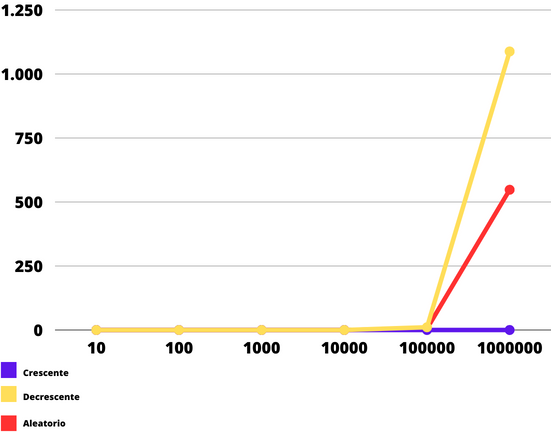
\includegraphics[width = 10cm]{Imagens/Insertion Sort/graficocanvas.png}
    \caption{Gráfico de tempo do algoritmo Inserion Sort. }
    \label{grafico_insert}
\end{figure}




        \newpage
        \subsection{Selection Sort}
		\begin{table}[h]
    \centering
    \caption{Comparação do Tempo do Seletion Sort}
    \begin{tabular}{|c|c|c|c|c|c|c|}
        \hline
        Tamanho de Entrada & 10 & 100 & 1000 & 10000 & 100000 & 1000000 \\
        \hline
        Crescente & 0.000000 & 0.000000 & 0.001000 & 0.103000 & 10.177000 & 1089.101000 \\
        \hline
        Decrescente & 0.000000 & 0.000000 & 0.000000 & 0.098000 & 9.769000 & 1046.444000 \\
        \hline
        Aleatória & 0.000000 & 0.000000 & 0.000000 & 0.102000 & 10.196000 & 1055.879000 \\
        \hline
    \end{tabular}
    \label{tab:comparacaoinsert}
\end{table}

Para a elaboração da tabela (Tabela \ref{tab:comparacaoinsert}) e do gráfico (Figura \ref{fig:select1}), foi desenvolvido um algoritmo em C com o intuito de gerar arquivos de diferentes tamanhos de entrada, 10, 100, 1.000, 10.000, 100.000 ou 1.000.000, contendo sequências de números, bem como seus n sucessores. Essas sequências puderam ser geradas em ordem Crescente, Decrescente ou Aleatória. Os resultados obtidos revelam características do funcionamento do Selection Sort. Este algoritmo demonstra consistência em sua performance, apresentando resultados similares em diferentes cenários de entrada. O Selection Sort tem uma performance homogênea e previsível, independentemente de o conjunto de dados estar ordenado, parcialmente ordenado ou em ordem inversa.

\begin{figure}[h!]
    \centering
    \includegraphics[width = 10cm]{Imagens/Selection Sort/Captura de Tela 2023-09-27 às 18.27.08.png}
    \caption{Gráfico de tempo do algoritmo Selection Sort.}
    \label{fig:select1}
\end{figure}
        \newpage
        \subsection{Shell Sort}
		\begin{table}[h]
    \centering
    \caption{Comparação do Tempo do Shell Sort}
    \begin{tabular}{|c|c|c|c|c|c|c|}
        \hline
        Tamanho de Entrada & 10 & 100 & 1000 & 10000 & 100000 & 1000000 \\
        \hline
        Crescente & 0.000000 & 0.000000 & 0.000000 & 0.000000 & 0.004000 & 0.063000 \\
        \hline
        Decrescente & 0.000000 & 0.000000 & 0.000000 & 0.001000 & 0.007000 & 0.083000 \\
        \hline
        Aleatória & 0.000000 & 0.000000 & 0.000000 & 0.001000 & 0.022000 & 0.300000 \\
        \hline
    \end{tabular}
    \label{tab:comparacaoshell}
\end{table}

A Tabela \ref{tab:comparacaoshell} mostra o Bubble Sort nos 6 diferentes tamanhos
de entrada e 3 situações diferentes de como as entradas são postas em determinados arquivos. Os resultados mostram que o algoritmo executa muito rápido até para entradas muito grande. Diferentemente dos algoritmos de ordenação mais simples, como Bubble Sort e Selection Sort, o Shell Sort emprega uma estratégia de redução de intervalo para melhorar a eficiência do Insertion Sort, conseguindo assim lidar com conjuntos de dados mais amplos de maneira mais eficaz. Mesmo na forma aleatória ter sido maior que as demais com muitas entradas, é um valor insignificante pois não passa de um segundo de execução.

\begin{figure}[h!]
    \centering
    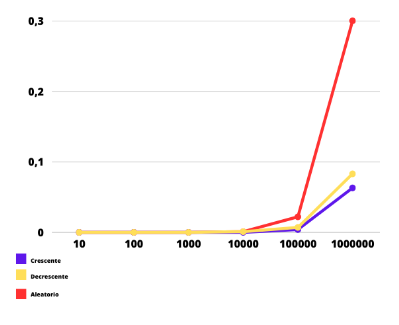
\includegraphics[width = 10cm]{Imagens/Shell Sort/Captura de tela 2023-09-27 211633.png}
    \caption{Gráfico de tempo do algoritmo Shell Sort.}
    \label{fig:shell1}
\end{figure}
        \newpage
        \subsection{Bubble Sort}
		\begin{table}[h]
    \centering
    \caption{Comparação do Tempo do Bubble Sort}
    \begin{tabular}{|c|c|c|c|c|c|c|}
        \hline
        Tamanho de Entrada & 10 & 100 & 1000 & 10000 & 100000 & 1000000 \\
        \hline
        Crescente & 0.000000 & 0.000000 & 0.001000 & 0.098000 & 9.734000 & 952.523000 \\
        \hline
        Decrescente & 0.000000 & 0.000000 & 0.002000 & 0.172000 & 17.373000 & 1697.082000 \\
        \hline
        Aleatória & 0.000000 & 0.000000 & 0.001000 & 0.212000 & 25.232000 & 2665.916000 \\
        \hline
    \end{tabular}
    \label{tab:comparacaobubble}
\end{table}

A Tabela \ref{tab:comparacaobubble} mostra o Bubble Sort nos 6 diferentes tamanhos
de entrada e 3 situações diferentes de como as entradas são postas em determinados arquivos, assim como os demais algoritmos.Os resultados evidenciaram certas características fundamentais do algoritmo Bubble Sort. Este algoritmo exibe uma performance uniforme e estável, gerando resultados semelhantes em diversas condições de entrada. O Bubble Sort, devido à sua abordagem de comparação e troca sequencial, não se beneficia substancialmente de dados parcialmente ordenados e, consequentemente, sua eficiência é consideravelmente constante, independentemente do estado inicial dos dados, mesmo com esse resultado ele ter demorado mais na forma aleatória, o médio caso dele possui a mesma complexidade dos demais.


\begin{figure}[h!]
    \centering
    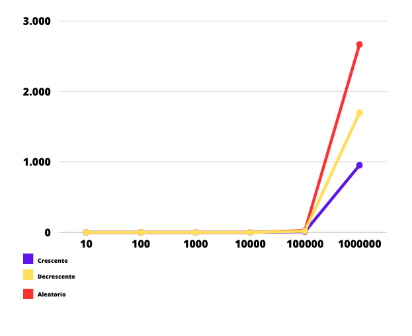
\includegraphics[width = 10cm]{Imagens/Bubble Sort/Captura de tela 2023-09-27 211808.png}
    \caption{Gráfico de tempo do algoritmo Merge Sort.}
    \label{fig:b10}
\end{figure}
        \newpage
        \subsection{Merge Sort}
		\begin{table}[h]
    \centering
    \caption{Comparação do Tempo do Insertion Sort}
    \begin{tabular}{|c|c|c|c|c|c|c|}
        \hline
        Tamanho de Entrada & 10 & 100 & 1000 & 10000 & 100000 & 1000000 \\
        \hline
        Crescente & 0.000000 & 0.000000 & 0.000000 & 0.000000 & 0.008000 & 0.100000 \\
        \hline
        Decrescente & 0.000000 & 0.000000 & 0.000000 & 0.001000 & 0.008000 & 0.099000 \\
        \hline
        Aleatória & 0.000000 & 0.000000 & 0.000000 & 0.001000 & 0.014000 & 0.173000 \\
        \hline
    \end{tabular}
    \label{tab:comparacao}
\end{table}

A Tabela mostra o Merge Sort nos 6 diferentes tamanhos de entrada e 3 situações diferentes de como as entradas são postas em determinados arquivos, assim como os demais algoritmos. Os resultados evidenciaram certas características fundamentais do algoritmo Merge Sort. Este algoritmo exibe uma performance uniforme e estável, gerando resultados semelhantes em diversas condições de entrada. O Merge Sort, devido à sua abordagem de divisão e conquista, mantém uma performance consistente, independentemente do estado inicial dos dados. Isso o torna eficiente tanto para dados ordenados quanto para dados parcialmente ordenados. Em média, o Merge Sort mantém uma complexidade de tempo O(n log n), tornando-o uma escolha sólida para ordenação em cenários de grande escala e em diferentes configurações de dados.

 \begin{figure}[H]
    \centering
    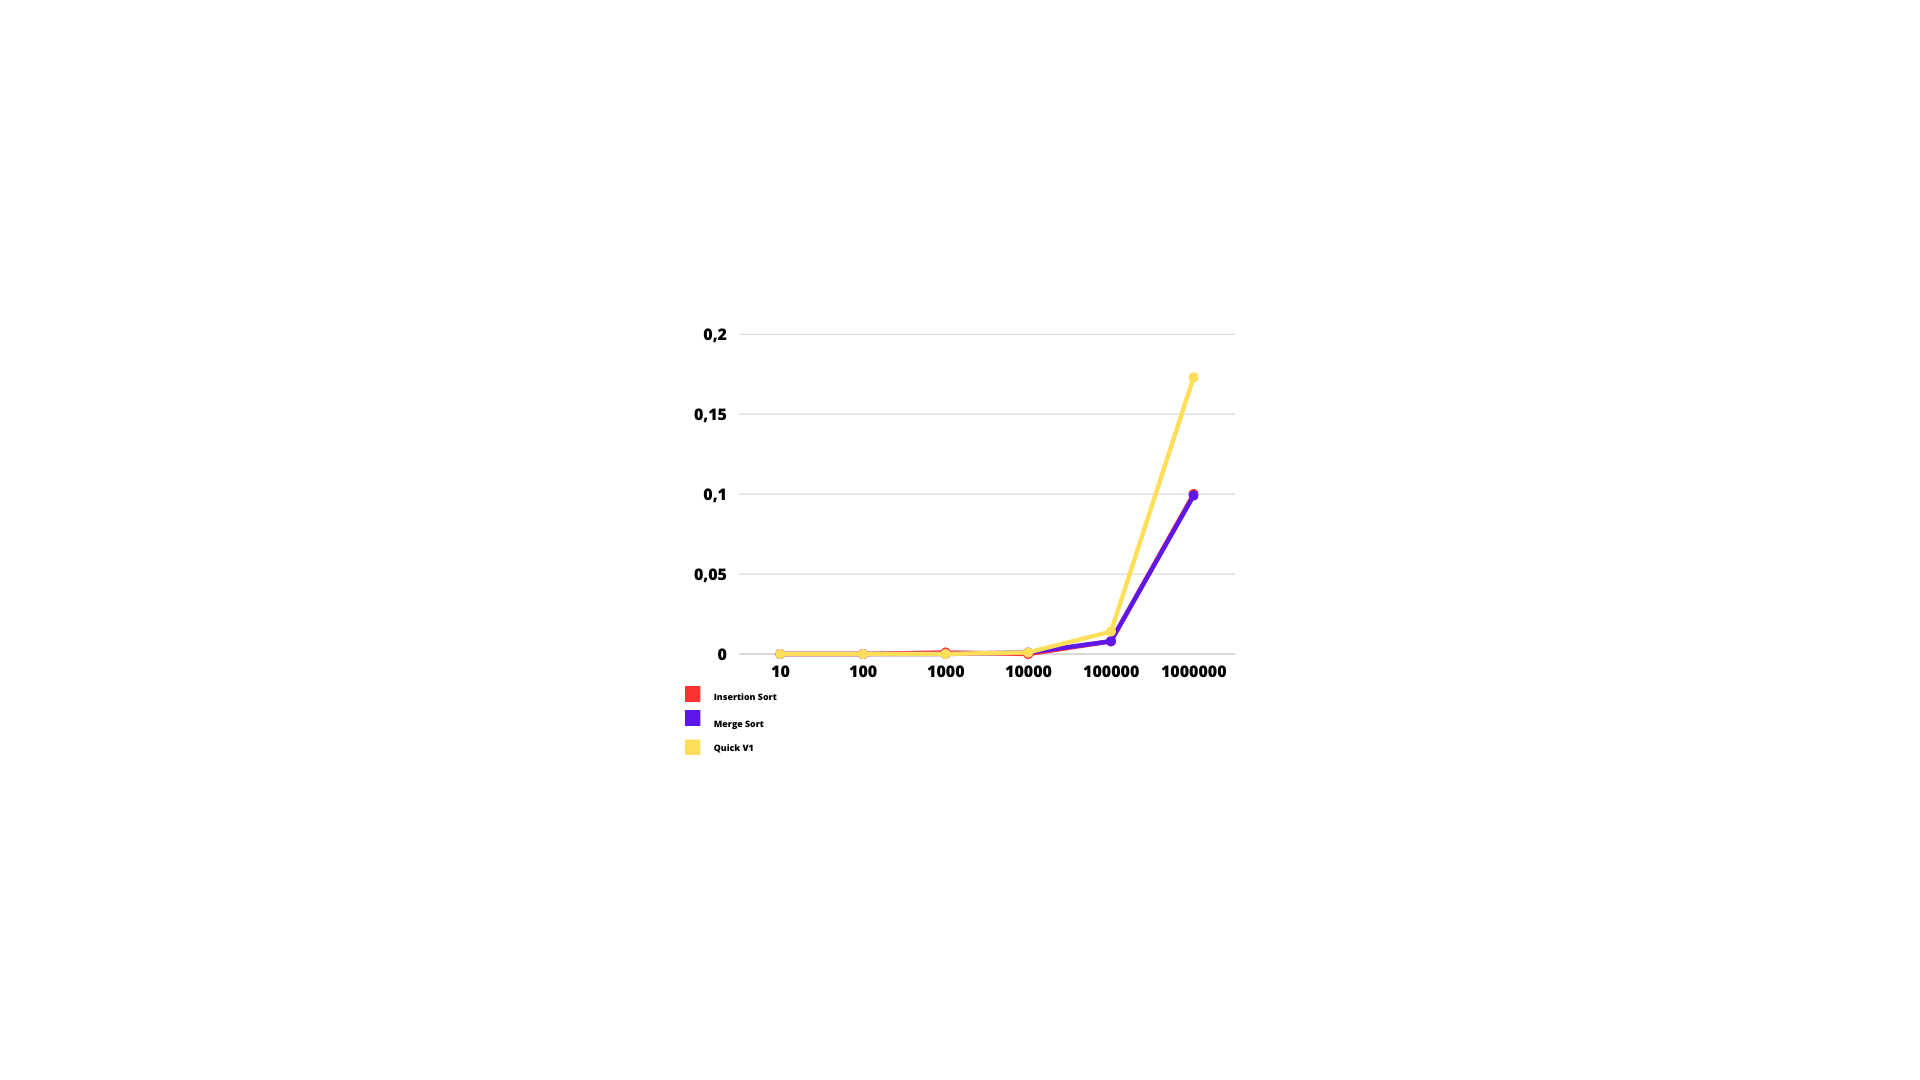
\includegraphics[width = 20cm]{Imagens/Merge Sort/merge.png}
    \caption{Gráfico de tempo do Merge Sort. }
    \label{imagem_digrama}
\end{figure}



        \newpage
        \subsection{Insertion X Merge X Quick Sort}
		\begin{table}[h]
    \centering
    \caption{Comparação do Tempo do Insertion Sort, Merge Sort e Quick Sort}
    \begin{tabular}{|c|c|c|c|c|c|c|}
        \hline
        Tamanho de Entrada & 10 & 100 & 1000 & 10000 & 100000 & 1000000 \\
        \hline
        Insertion & 0.000000 & 0.000000 & 0.001000 & 0.103000 & 10.177000 & 1089.101000 \\
        \hline
        Merge & 0.000000 & 0.000000 & 0.000000 & 0.001000 & 0.008000 & 0.099000 \\
        \hline
        QuickV1 & 0.000000 & 0.000000 & 0.002000 & 0.139000 & 14.307000 & 1456.626000 \\
        \hline
        QuickV2 & 0.000000 & 0.000000 & 0.000000 & 0.000000 & 6.522145 & 1240.6443000 \\
        \hline
        QuickV3 & 0.000000 & 0.000000 & 0.000000 & 0.001000 & 7.0014000 & 151.0000230\\
        \hline
        QuickV4 & 0.000000 & 0.000000 & 0.000000 & 0.000000 & 0.008000 & 0.316000 \\
        
        \hline
    \end{tabular}
    \label{tab:geralx}
\end{table}

Para a elaboração da tabela (Tabela \ref{tab:geralx}) e do gráfico (Figura \ref{fig:geralx1}), foi desenvolvido um algoritmo em C com o intuito de gerar arquivos de diferentes tamanhos de entrada, 10, 100, 1.000, 10.000, 100.000 ou 1.000.000, contendo sequências de números, bem como seus n sucessores. Essas sequências puderam ser geradas em ordem Crescente, Decrescente ou Aleatória. Os resultados obtidos revelam características do funcionamento do Insertion Sort, Merge Sort e Quick Sort. 

Observando a performance desses algoritmos, notamos que o Insertion Sort, embora simples e eficiente para pequenos conjuntos de dados ou conjuntos quase ordenados, tende a ser menos eficaz em entradas maiores, onde seu desempenho se deteriora. O Merge Sort, por outro lado, mantém uma performance estável e eficaz, independentemente da configuração inicial dos dados. Ele é particularmente eficiente em ordenar grandes volumes de dados e é conhecido por sua complexidade de tempo O(n log n). 

O Quick Sort se destaca por sua velocidade média, especialmente em entradas desordenadas, graças ao seu processo de divisão e conquista. No entanto, sua performance pode variar dependendo da escolha do pivô e da configuração dos dados, o que o torna menos previsível em alguns casos. No geral, o Merge Sort e o Quick Sort são frequentemente preferidos em cenários de ordenação de grande escala, devido à sua eficiência em comparação com o Insertion Sort.



\begin{figure}[H]
    \centering
    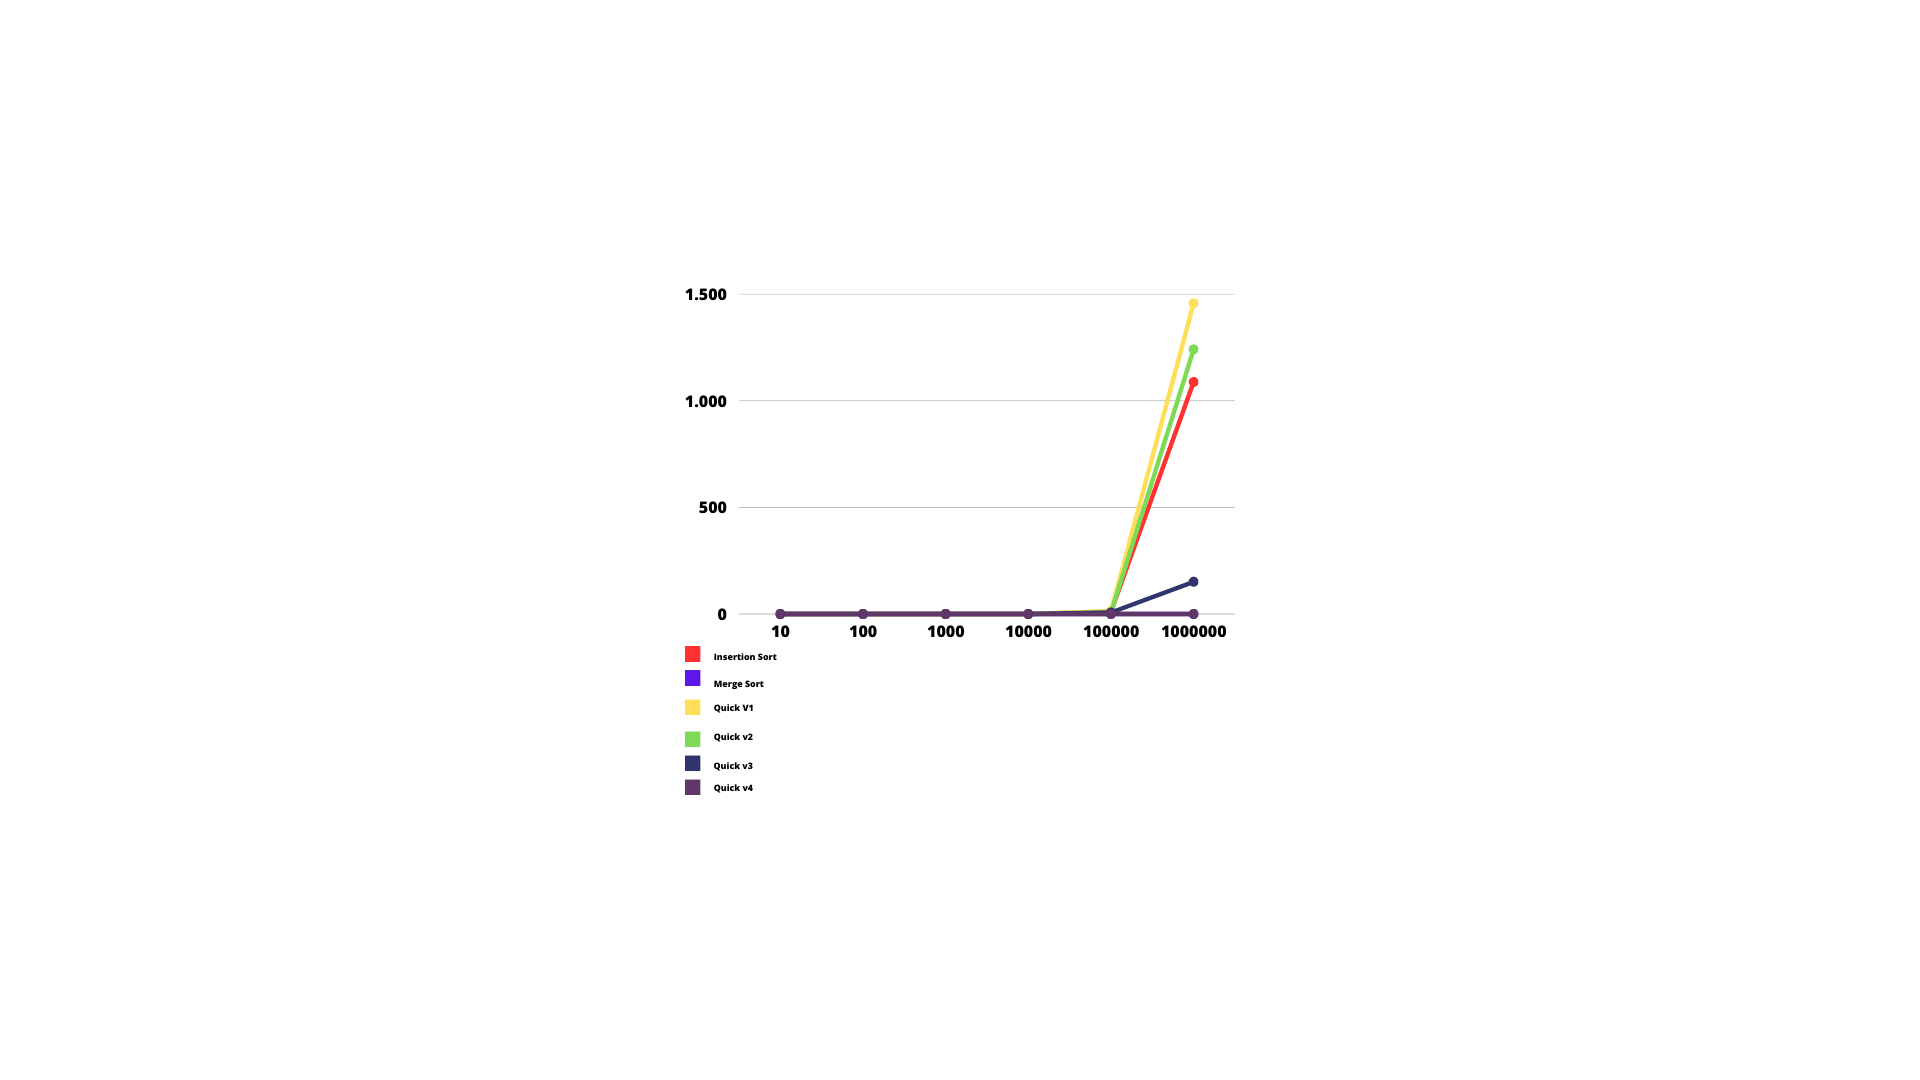
\includegraphics[width = 20cm]{Imagens/Quickx Sort/graficogeral.png}
    \caption{Gráfico de tempo do algoritmo Insertion Sort, Merge Sort e Quick Sort.}
    \label{fig:geralx1}
\end{figure}
        \subsection{HeapSort}
		\begin{table}[h]
    \centering
    \caption{Comparação do Tempo do HeapSort}
    \begin{tabular}{|c|c|c|c|c|c|c|}
        \hline
        Tamanho de Entrada & 10 & 100 & 1000 & 10000 & 100000 & 1000000 \\
        \hline
        Crescente & 0.000000 & 0.000000 & 0.000000 & 0.002000 & 0.018000 & 0.212000 \\
        \hline
        Decrescente & 0.000000 & 0.000000 & 0.000000 & 0.002000 & 0.018000 & 0.215000 \\
        \hline
        Aleatória & 0.000000 & 0.000000 & 0.000000 & 0.001000 & 0.023000 & 0.318000 \\
        \hline
    \end{tabular}
    \label{tab:comparacaobubble}
\end{table}

A tabela apresenta a performance do algoritmo Heap Sort em seis diferentes tamanhos de entrada e em três situações distintas de ordenação dos dados: crescente, decrescente e aleatória. Os resultados demonstram as características notáveis do Heap Sort, um algoritmo eficiente para criar uma estrutura de dados de heap e realizar a ordenação.

Observa-se que, para entradas de pequeno tamanho (10 e 100), o tempo de execução é insignificante, refletindo a eficiência do algoritmo em lidar com conjuntos de dados menores. À medida que o tamanho da entrada aumenta, nota-se um crescimento gradual no tempo de execução, o que é esperado dada a complexidade de tempo O(n log n) do Heap Sort.

As variações entre os tempos para entradas crescentes, decrescentes e aleatórias são mínimas, indicando que o Heap Sort não é sensivelmente afetado pela ordenação inicial dos dados. Isso contrasta com algoritmos como o Bubble Sort, que pode ter um desempenho pior em entradas decrescentes.

O Heap Sort mostra-se, portanto, como um algoritmo robusto e confiável, com bom desempenho consistente em diferentes cenários. Sua capacidade de manter uma performance estável o torna uma opção viável para aplicações onde os dados podem ser apresentados em qualquer ordem e onde o tempo de execução previsível é crítico.

 \begin{figure}[H]
    \centering
    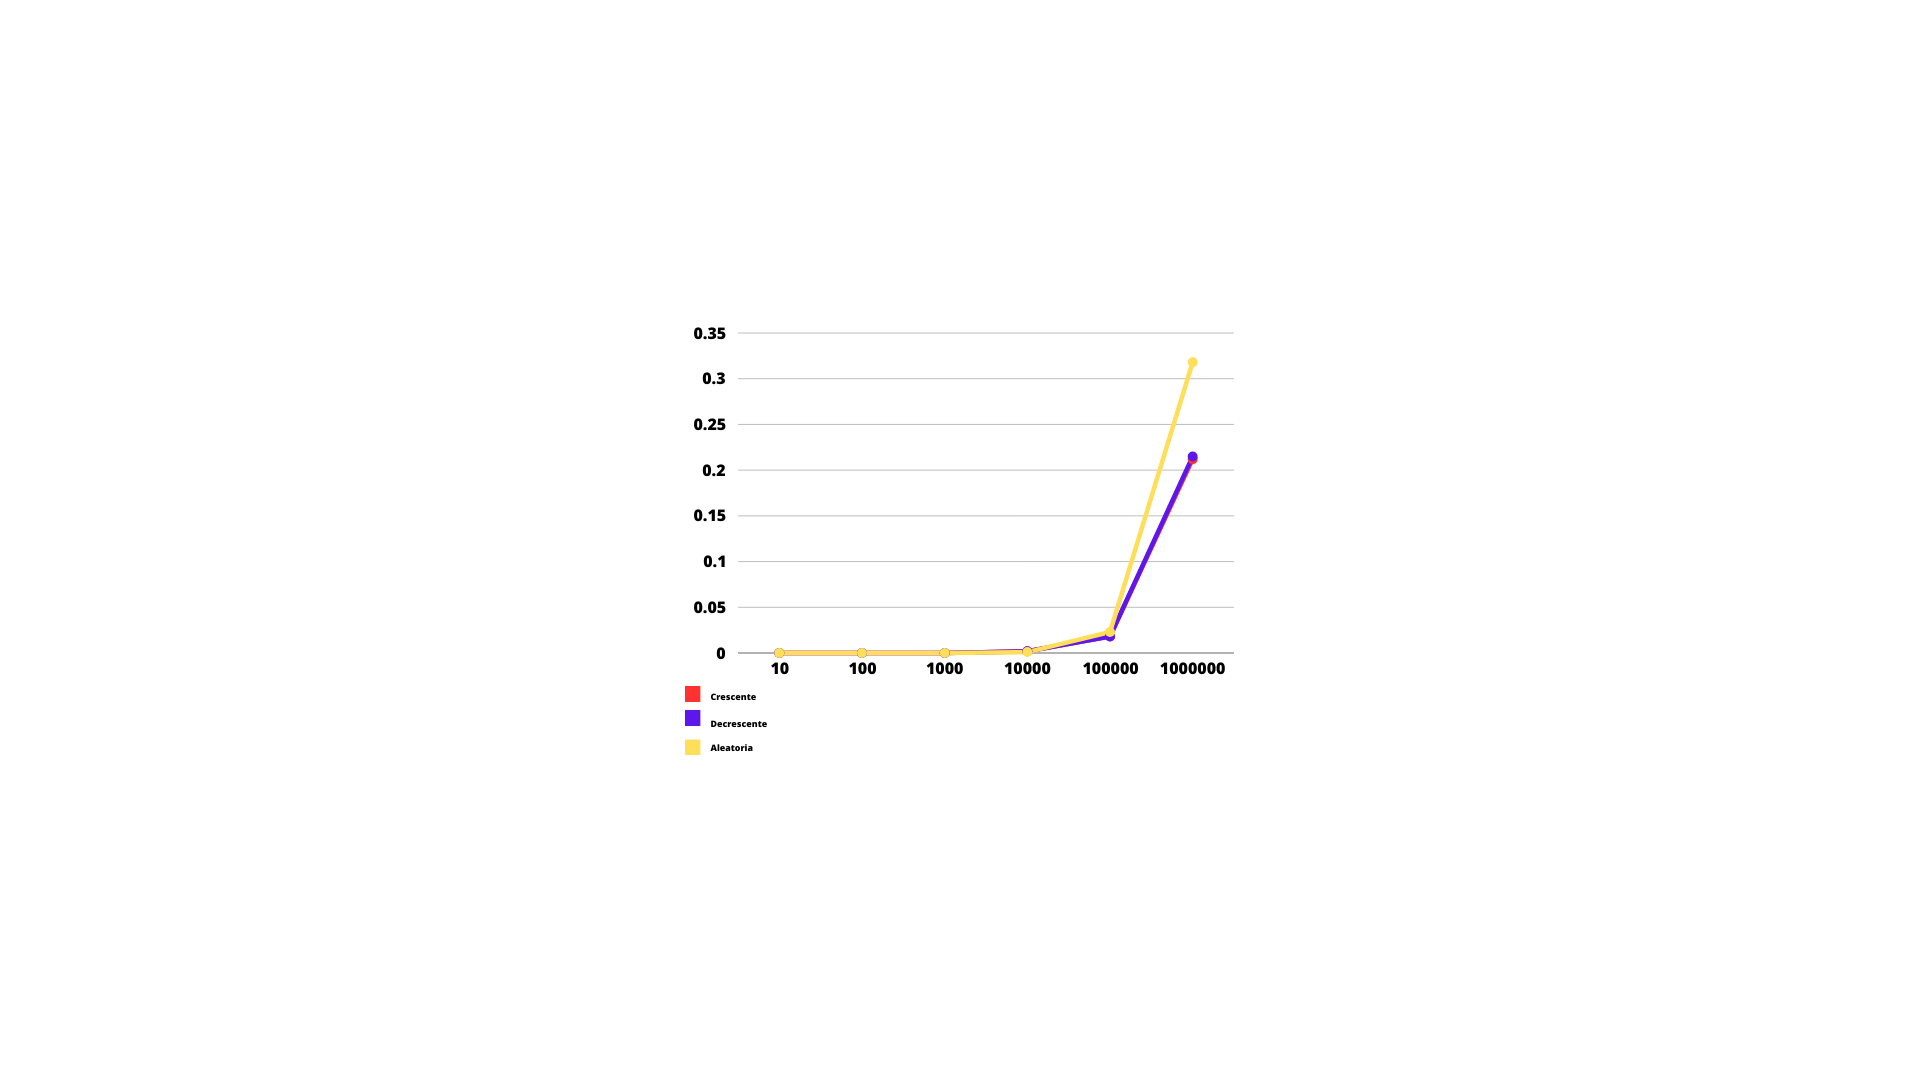
\includegraphics[width = 20cm]{Imagens/Heap Sort/zz.png}
    \caption{Gráfico de tempo do HeapSort. }
    \label{imagem_digrama}
\end{figure}

        \newpage
        \subsection{Geral}
		\begin{table}[h]
    \centering
    \caption{Comparação do Tempo entre os algoritmos com entrada crescente.}
    \begin{tabular}{|c|c|c|c|c|c|c|}
        \hline
        Tamanho de Entrada & 10 & 100 & 1000 & 10000 & 100000 & 1000000 \\
        \hline
        Insertion Sort & 0.000000 & 0.000000 & 0.000000 & 0.000000 & 0.000000 & 0.003000 \\
        \hline
        Selection Sort & 0.000000 & 0.000000 & 0.001000 & 0.103000 & 10.177000 & 1089.101000 \\
        \hline
        Shell Sort & 0.000000 & 0.000000 & 0.000000 & 0.000000 & 0.004000 & 0.063000 \\
        \hline
        Bubble Sort & 0.000000 & 0.000000 & 0.001000 & 0.098000 & 9.734000 & 952.523000 \\
        \hline
    \end{tabular}
    \label{tab:comparacaogeral}
\end{table}

Observando à Tabela \ref{tab:comparacaogeral} e o gráfico \ref{fig:geral1} percebemos que quando se trata da entrada no melhor caso, ou seja, com números já ordenados, os algoritmos Insertion Sort e Shell sort continuam tendo uma boa performance até mesmo com valores muito altos de entrada, permanecendo com o tempo de ordenação próximo ao zero, já o Selection Sort e o Bubble sorte, mantém um bom tempo de execução com valores baixo mas quando se trata de muitas entradas eles gastam muito tempo para percorrer todo o vetor, pois mesmo já estando alternados os números eles precisam conferir todos até o final, não sendo uma boa escolha.

\begin{figure}[h!]
    \centering
    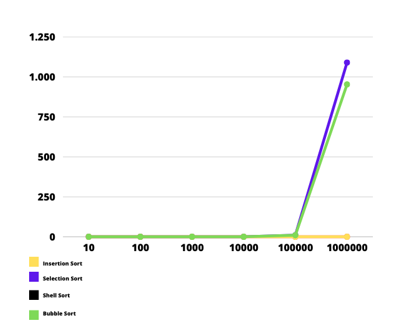
\includegraphics[width = 10cm]{Imagens/Geral/geral2.png}
    \caption{Gráfico de tempo entre os algoritmos com entrada crescente.}
    \label{fig:geral1}
\end{figure}
\newpage

\begin{table}[h]
    \centering
    \caption{Comparação do Tempo entre os algoritmos com entrada decrescente.}
    \begin{tabular}{|c|c|c|c|c|c|c|}
        \hline
        Tamanho de Entrada & 10 & 100 & 1000 & 10000 & 100000 & 1000000 \\
        \hline
        Insertion Sort & 0.000000 & 0.000000 & 0.001000 & 0.111000 & 10.856000 & 1088.031000 \\
        \hline
        Selection Sort & 0.000000 & 0.000000 & 0.000000 & 0.098000 & 9.769000 & 1046.444000 \\
        \hline
        Shell Sort & 0.000000 & 0.000000 & 0.000000 & 0.001000 & 0.007000 & 0.083000 \\
        \hline
        Bubble Sort & 0.000000 & 0.000000 & 0.002000 & 0.172000 & 17.373000 & 1697.082000 \\
        \hline
    \end{tabular}
    \label{tab:comparacaogeral2}
\end{table}

Enquanto para o pior caso, na Tabela \ref{tab:comparacaogeral2}, o único algoritmo que apresente uma diferença relevante com o melhor caso, é o Insertion Sort, que precisa percorrer e inverter todo o vetor para ordenar todos os números, tornando-o assim uma escolha inviável para entradas descrescentes quando se trata de um grande número de entradas no algoritmo.

\begin{figure}[h!]
    \centering
    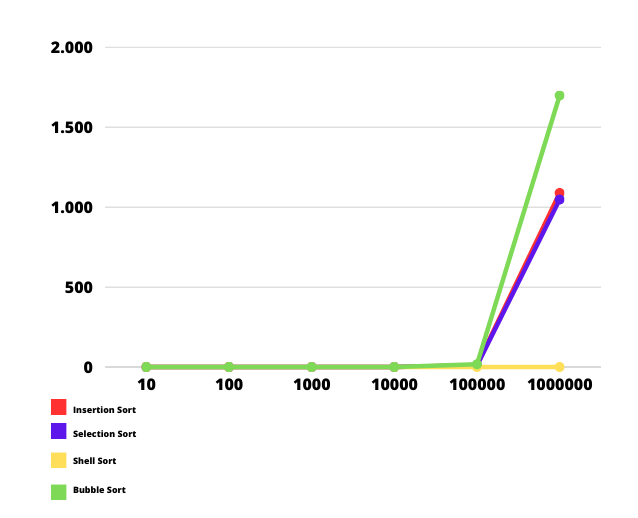
\includegraphics[width = 10cm]{Imagens/Geral/Captura de tela 2023-09-27 220558.png}
    \caption{Gráfico de tempo entre os algoritmos com entrada decrescente.}
    \label{fig:geral2}
\end{figure}
\newpage

		\newpage
  
		\section{CONCLUSÃO}
		Este estudo empreendeu uma avaliação comparativa abrangente de sete algoritmos de ordenação: Insertion Sort, Selection Sort, Bubble Sort, Shell Sort, Merge Sort, Quick Sort e Heap Sort. Cada um foi examinado sob o prisma de seus fundamentos teóricos e eficácia operacional em uma gama de condições de entrada - sequências crescentes, decrescentes e aleatórias - em seis diferentes tamanhos de conjuntos de dados.

A análise revelou características singulares inerentes a cada algoritmo. O Insertion Sort se sobressaiu em conjuntos menores e quase ordenados, mas sua performance declinou consideravelmente sob a pressão de volumes maiores e desordem generalizada, onde a natureza quadrática de seu desempenho se tornou aparente. Por outro lado, o Selection Sort e o Bubble Sort mantiveram um comportamento previsível, enquanto o Merge Sort e o Quick Sort mostraram-se eficazes e estáveis, com tempos de execução que escalavam proporcionalmente à complexidade O(n log n), independentemente da ordenação inicial dos dados.

O Shell Sort destacou-se pela sua estratégia de ordenação por intervalos, exibindo eficiência notável em dados volumosos e desorganizados, destacando-se como uma opção versátil e eficaz. A performance do Heap Sort também foi notável, especialmente pela sua capacidade de manter uma eficiência consistente em todas as condições testadas, validando sua complexidade de tempo O(n log n) e sua viabilidade como método de ordenação para grandes volumes de dados.

Os gráficos inclusos neste trabalho proporcionaram uma compreensão visual intuitiva das diferenças de desempenho entre os algoritmos, confirmando os achados teóricos e experimentais. Estas representações gráficas serviram não apenas para validar as observações analíticas mas também para aprimorar o entendimento geral da eficácia comparativa e das limitações intrínsecas a cada técnica de ordenação.

Em resumo, este trabalho destacou as forças e as fraquezas de cada algoritmo de ordenação estudado, ilustrando sua adequação para contextos variados. O Insertion Sort provou ser simples e eficiente para conjuntos menores ou quase ordenados; o Selection Sort e o Bubble Sort foram consistentes e previsíveis; o Merge Sort e o Quick Sort mostraram-se robustos e confiáveis para qualquer ordenação de entrada; o Shell Sort foi adaptável e eficaz para grandes volumes de dados; e o Heap Sort confirmou sua posição como uma solução confiável e eficiente, especialmente em aplicações onde a previsibilidade e a estabilidade são cruciais. A escolha do algoritmo mais apropriado deve, portanto, ser informada pelas especificidades e exigências de cada aplicação individual.
		\newpage
  
		\section{REFERÊNCIAS BIBLIOGRÁFICAS}
		\bibliographystyle{plain}
        \bibliography{referencias}
        \include{file}

        	
\end{document}